\documentclass[11pt,t,usepdftitle=false,aspectratio=169]{beamer}
%% ------------------------------------------------------------------
%% - aspectratio=43: Set paper aspect ratio to 4:3.
%% - aspectratio=169: Set paper aspect ratio to 16:9.
%% ------------------------------------------------------------------

%% Add packages
\usepackage{eso-pic}
\usepackage{graphics}


\usetheme[nototalframenumber,foot,logo]{uibk}
%% ------------------------------------------------------------------
%% - foot: Add a footer line for conference name and date.
%% - logo: Add the university logo in the footer (only if 'foot' set).
%% - bigfoot/sasquatch: Larger font size in footer.
%% - nototalslidenumber: Hide the total number of slides (only if 'foot' set)
%% - license: Add CC-BY license symbol to title slide (e.g., for conference uploads)
%%   (TODO: At the moment no other licenses are supported.)
%% - licenseall: Add CC-BY license symbol to all subsequent slides slides
%% - url: use \url{} rather than \href{} on the title page
%% ------------------------------------------------------------------

%% Set the size of the footer text
\setbeamerfont{footline}{size*={6pt}{6pt},parent=normal text}

%% ------------------------------------------------------------------
%% The official corporate colors of the university are predefined and
%% can be used for e.g., highlighting something. Simply use
%% \color{uibkorange} or \begin{color}{uibkorange} ... \end{color}
%% Defined colors are:
%% - uibkblue, uibkbluel, uibkorange, uibkorangel, uibkgray, uibkgraym, uibkgrayl
%% The frametitle color can be easily adjusted e.g., to black with
%% \setbeamercolor{titlelike}{fg=black}
%% ------------------------------------------------------------------

\setbeamercolor{verbcolor}{fg=uibkorange}

%% ------------------------------------------------------------------
%% Setting a highlight color for verbatim output such as from
%% the commands \pkg, \email, \file, \dataset 
%% ------------------------------------------------------------------


%% information for the title page ('short title' is the pdf-title that is shown in viewer's titlebar)
\title[HyPA]{HyPA: A Hybrid Pod Autoscaler}
\subtitle{Autoscaling of container-orchestration environments for enhanced VoIP performance}

%('short author' is the pdf-metadata Author)
%% If multiple authors are required and the font size is too large you
%% can overrule the font size of author and url by calling:
%\setbeamerfont{author}{size*={10pt}{10pt},series=\mdseries}
%\setbeamerfont{url}{size*={10pt}{10pt},series=\mdseries}
\author[Dominik Gratz \& René Hueber]{Dominik Gratz, René Hueber\\[3mm]{\small Supervisors: Zahra Najafabadi Samani, PhD \\ \hspace{20mm} Juan Aznar Poveda, PhD}}


\footertext{Department of Computer Science \space - \space Bachelor Thesis \space - \space HyPA \space - \space June 18, 2024}

\headerimage{3}
%% ------------------------------------------------------------------
%% The theme offers four different header images based on the
%% corporate design of the university of innsbruck. Currently
%% 1, 2, 3 and 4 is allowed as input to \headerimage{...}. Default
%% or fallback is '1'.
%% ------------------------------------------------------------------


\begin{document}

%% ALTERNATIVE TITLEPAGE
%% The next block is how you add a titlepage with the 'nosectiontitlepage' option, which switches off
%% the default behavior of creating a titlepage every time a \section{} is defined.
%% Then you can use \section{} as it's originally intended, including a table of contents.
% \usebackgroundtemplate{\includegraphics[width=\paperwidth,height=\paperheight]{titlebackground.pdf}}
% \begin{frame}[plain]
%     \titlepage
% \end{frame}
% \addtocounter{framenumber}{-1}
% \usebackgroundtemplate{}}

%% Table of Contents, if wanted:
%% this requires the 'nosectiontitlepage' option and setting \section{}'s as you want them to appear here.
%% Subsections and subordinates are suppressed in the .sty at the moment, search
%% for \setbeamertemplate{subsection} and replace the empty {} with whatever you want.
%% Although it's probably too much for a presentation, maybe for a lecture.
% \begin{frame}
%     \vspace*{1cm plus 1fil}
%     \tableofcontents
%     \vspace*{0cm plus 1fil}
% \end{frame}


%% this sets the first PDF bookmark and triggers generation of the title page
\section{HyPA: A Hybrid Pod Autoscaler}

\subsection{Cooperation with World-Direct}
\begin{frame}
	\frametitle{Cooperation with {\color{uibkblue} World-Direct}}
	
	\AddToShipoutPicture*{\put(325,200){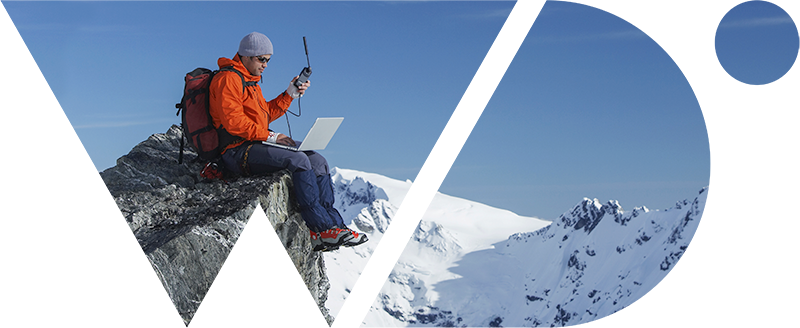
\includegraphics[width=4cm]{_images/world_direct_uc.png}}}
	
	\begin{itemize}
		\item Subsidiary company of A1
		\item Manages over 90.000 VoIP ports
		\item Transitions its telephone infrastructure to \textbf{\color{uibkorange} Kubernetes}
		\begin{itemize}
			\item Microservices
			\item API-first approach
			\item \textbf{{\color{uibkorange} Zero-Downtime}} architecture
		\end{itemize}
	\end{itemize}
\end{frame}

\begin{frame}
	\frametitle{Cooperation with {\color{uibkblue} World-Direct}}
	
	\AddToShipoutPicture*{\put(325,200){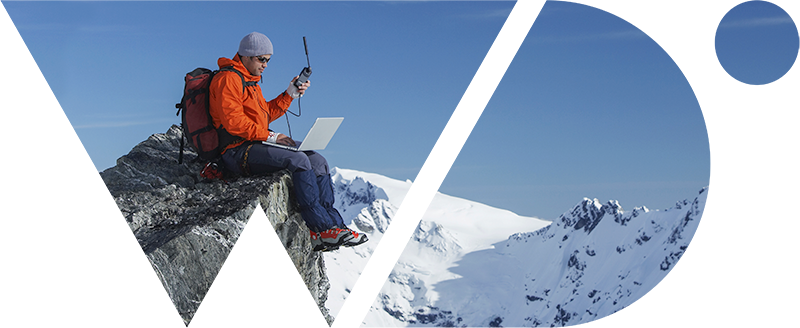
\includegraphics[width=4cm]{_images/world_direct_uc.png}}}
	
	\begin{itemize}
		\item Subsidiary company of A1
		\item Manages over 90.000 VoIP ports
		\item Transitions its telephone infrastructure to \textbf{\color{uibkorange} Kubernetes}
		\begin{itemize}
			\item Microservices
			\item API-first approach
			\item \textbf{{\color{uibkorange} Zero-Downtime}} architecture
		\end{itemize}
	\end{itemize}
	
	\begin{columns}
		\begin{column}{0.5\textwidth}		
			\begin{block}{Pros}
				\begin{itemize}
					\item Less complexity on the client side
					\item Central maintenance
					\item High flexibility and \textbf{\color{uibkorange} scalability}
				\end{itemize}
			\end{block}
		\end{column}
		
		\begin{column}{0.5\textwidth}
		\end{column}
	\end{columns}
\end{frame}

\begin{frame}
	\frametitle{Cooperation with {\color{uibkblue} World-Direct}}
	
	\AddToShipoutPicture*{\put(325,200){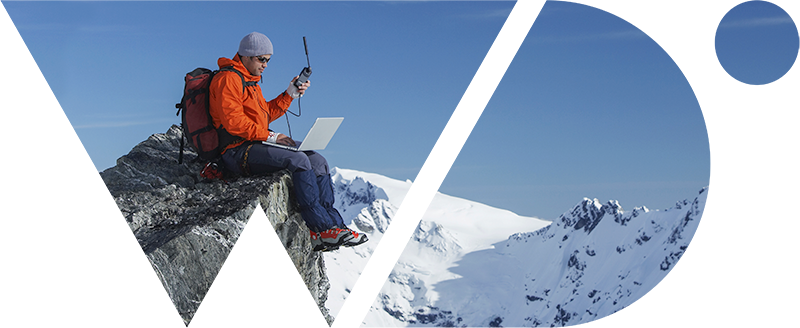
\includegraphics[width=4cm]{_images/world_direct_uc.png}}}
	
	\begin{itemize}
		\item Subsidiary company of A1
		\item Manages over 90.000 VoIP ports
		\item Transitions its telephone infrastructure to \textbf{\color{uibkorange} Kubernetes}
		\begin{itemize}
			\item Microservices
			\item API-first approach
			\item \textbf{{\color{uibkorange} Zero-Downtime}} architecture
		\end{itemize}
	\end{itemize}
	
	\begin{columns}
		\begin{column}{0.5\textwidth}		
			\begin{block}{Pros}
				\begin{itemize}
					\item Less complexity on the client side
					\item Central maintenance
					\item High flexibility and \textbf{\color{uibkorange} scalability}
				\end{itemize}
			\end{block}
		\end{column}
		
		\begin{column}{0.5\textwidth}		
			\begin{block}{Cons}
				\begin{itemize}
					\item Complex infrastructure
					\item Efficient architectures necessary
					\item \textbf{\color{red} Timely scaling}
				\end{itemize}
			\end{block}
		\end{column}
	\end{columns}
\end{frame}

\subsection{Problem formulation: Scaling realtime applications}
\begin{frame}
	\frametitle{Problem formulation: Scaling {\color{uibkorange} realtime} applications}
	
	\begin{itemize}
		\item Challenges in VoIP:
		\begin{itemize}
			\item \textbf{\color{uibkorange} Stateful} protocols
			\item Time-sensitive signaling
			\item Sessions over a long period of time
		\end{itemize}
	\end{itemize}
\end{frame}

\begin{frame}
	\frametitle{Problem formulation: Scaling {\color{uibkorange} realtime} applications}
	
	\begin{itemize}
		\item Challenges in VoIP:
		\begin{itemize}
			\item \textbf{\color{uibkorange} Stateful} protocols
			\item Time-sensitive signaling
			\item Sessions over a long period of time
		\end{itemize}
		
		\item High call volume traffic: 
		\begin{itemize}
			\item Increased load on the telephone system core
			\item Increased latency
			\item Call failures
		\end{itemize}
	\end{itemize}
\end{frame}

\begin{frame}
	\frametitle{Problem formulation: Scaling {\color{uibkorange} realtime} applications}
	
	\begin{itemize}
		\item Challenges in VoIP:
		\begin{itemize}
			\item \textbf{\color{uibkorange} Stateful} protocols
			\item Time-sensitive signaling
			\item Sessions over a long period of time
		\end{itemize}
		
		\item High call volume traffic: 
		\begin{itemize}
			\item Increased load on the telephone system core
			\item Increased latency
			\item Call failures
		\end{itemize}
		
		\item \textbf{\color{uibkorange} Default Kubernetes} scaling is not enough:
		\begin{itemize}
			\item Static thresholds
			\item Limited option for custom parameters
			\item No hybrid scaling approach
		\end{itemize}
	\end{itemize}
\end{frame}

\subsection{Thesis goal}
\begin{frame}
	\frametitle{Thesis goal}
	
	\begin{block}{\textbf{HyPA}}
		\begin{itemize}
			\item \textbf{\color{uibkorange} Hy}brid scaling:
			\begin{itemize}
				\item Horizontal $\rightarrow$ variable number of replicas (pods)
				\item Vertical $\rightarrow$ variable CPU/memory assignment of a pod
			\end{itemize}

			\item \textbf{\color{uibkorange} P}od \textbf{\color{uibkorange} A}utoscaling:
			\begin{itemize}
				\item Automatically scale service pods at runtime
			\end{itemize}
		\end{itemize}
	\end{block}
\end{frame}

\begin{frame}
	\frametitle{Thesis goal}
	
	\begin{block}{\textbf{HyPA}}
		\begin{itemize}
			\item \textbf{\color{uibkorange} Hy}brid scaling:
			\begin{itemize}
				\item Horizontal $\rightarrow$ variable number of replicas (pods)
				\item Vertical $\rightarrow$ variable CPU/memory assignment of a pod
			\end{itemize}
			
			\item \textbf{\color{uibkorange} P}od \textbf{\color{uibkorange} A}utoscaling:
			\begin{itemize}
				\item Automatically scale service pods at runtime
			\end{itemize}
		\end{itemize}
	\end{block}
	
	\begin{block}{\textbf{Challenges}}
		\begin{itemize}
			\item Maintain high call throughput with small latency
			\item Resource conservation
			\item Ensure no service downtime
		\end{itemize}
	\end{block}
\end{frame}

\begin{frame}
	\frametitle{Proposed Model}
	
	\begin{block}{Overview}
		\begin{itemize}
			\item RL learning approach
			\item Deployed in customer namespace
			\item Baseline model
			\item Focuses on CPU scaling
		\end{itemize}
	\end{block}
\end{frame}

\begin{frame}
	\frametitle{Proposed Model}
	
	\begin{block}{Overview}
		\begin{itemize}
			\item RL learning approach
			\item Deployed in customer namespace
			\item Baseline model
			\item Focuses on CPU scaling
		\end{itemize}
	\end{block}
	
	\begin{alertblock}{Model complexity reductions}
		\begin{itemize}
			\item No vertical memory scaling
			\item Discrete finite action space
		\end{itemize}
	\end{alertblock}
\end{frame}

\begin{frame}
	\frametitle{Infrastructure Model}
	
	\begin{figure}
		\centering
		\vspace*{-0.4cm}
		\includegraphics[width=12cm,height=7cm]{_images/infrastructure_model.png}
	\end{figure}
\end{frame}

\begin{frame}
	\frametitle{Model Training (1)}
	
	\begin{alertblock}{Call Data}
		\begin{itemize}
			\item No existing datasets
			\item Analyzed historic call data
			\item Cover \textbf{\color{red} all ranges} of clients
			\item Train a baseline model
		\end{itemize}
	\end{alertblock}
\end{frame}

\begin{frame}
	\frametitle{Model Training (1)}
	
	\begin{alertblock}{Call Data}
		\begin{itemize}
			\item No existing datasets
			\item Analyzed historic call data
			\item Cover \textbf{\color{red} all ranges} of clients
			\item Train a baseline model
		\end{itemize}
	\end{alertblock}
	
	\begin{block}{Call Generation}
		\begin{itemize}
			\item Based on real call patterns
			\item Custom scenarios utilizing \textbf{\color{uibkorange} SIPp}
		\end{itemize}
	\end{block}
\end{frame}

\begin{frame}
	\frametitle{Model Training (2)}
	
	\begin{figure}
		\centering
		\vspace*{-0.4cm}
		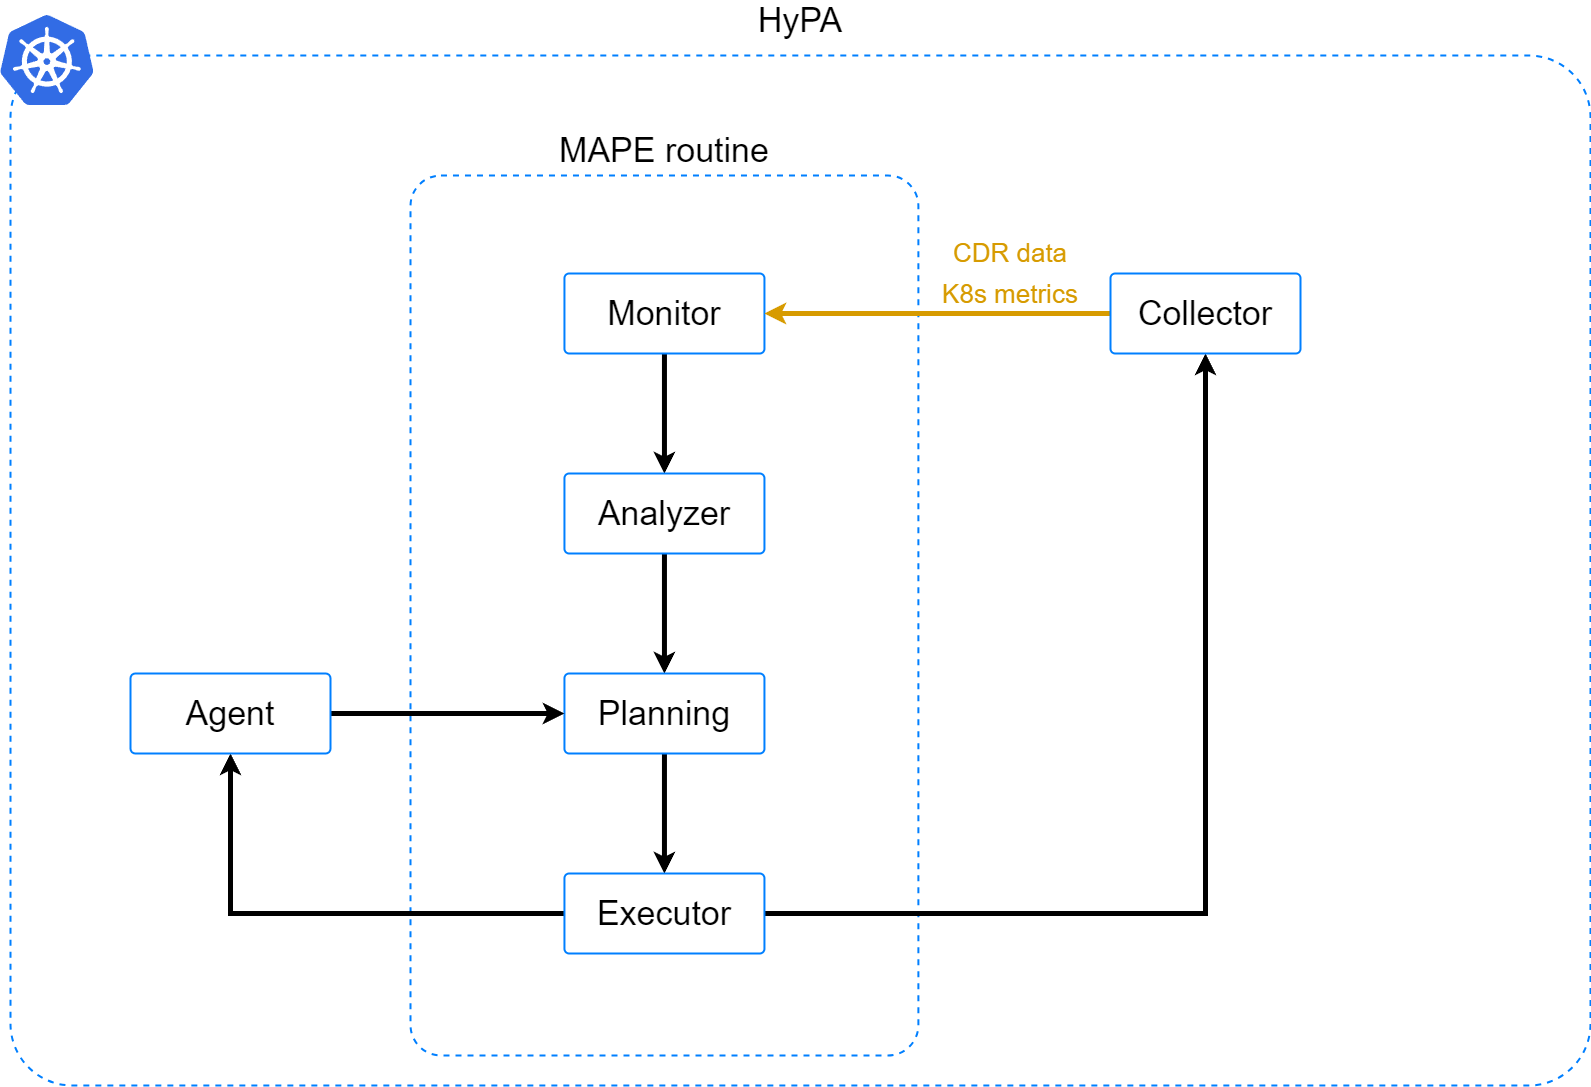
\includegraphics[width=12cm,height=7cm]{_images/trainings_model_1.png}
	\end{figure}
\end{frame}

\begin{frame}
	\frametitle{Model Training (3)}
	
	\begin{figure}
		\centering
		\vspace*{-0.4cm}
		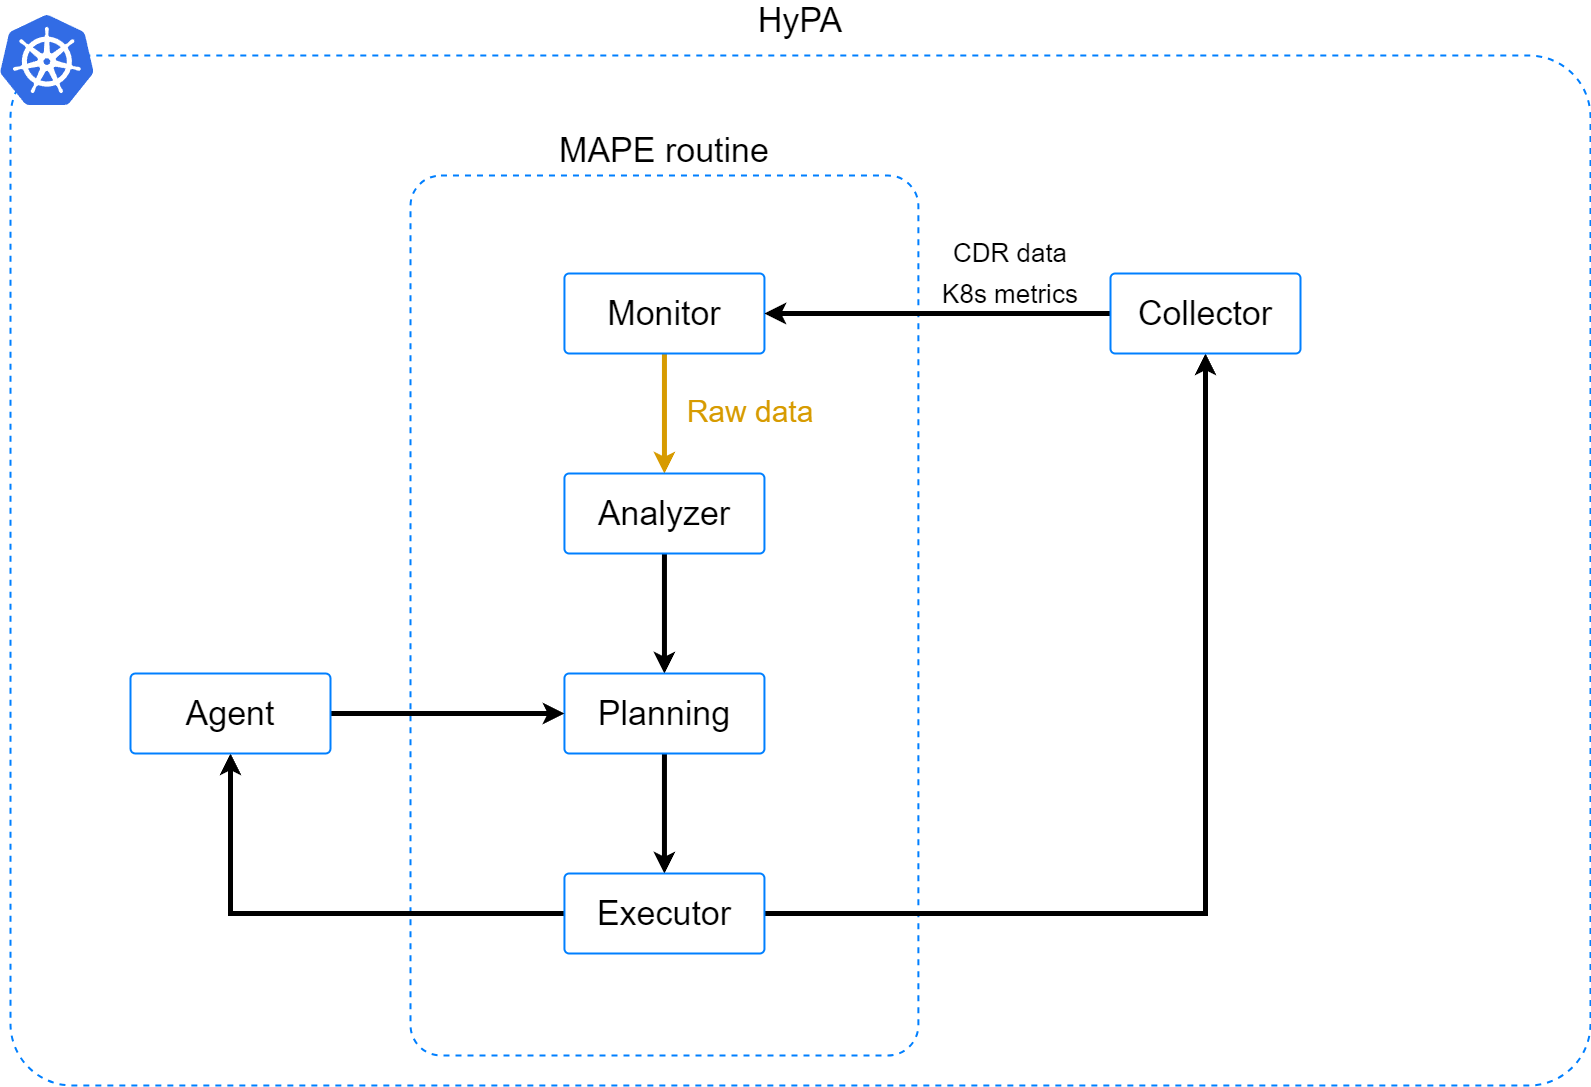
\includegraphics[width=12cm,height=7cm]{_images/trainings_model_2.png}
	\end{figure}
\end{frame}

\begin{frame}
	\frametitle{Model Training (4)}
	
	\begin{figure}
		\centering
		\vspace*{-0.4cm}
		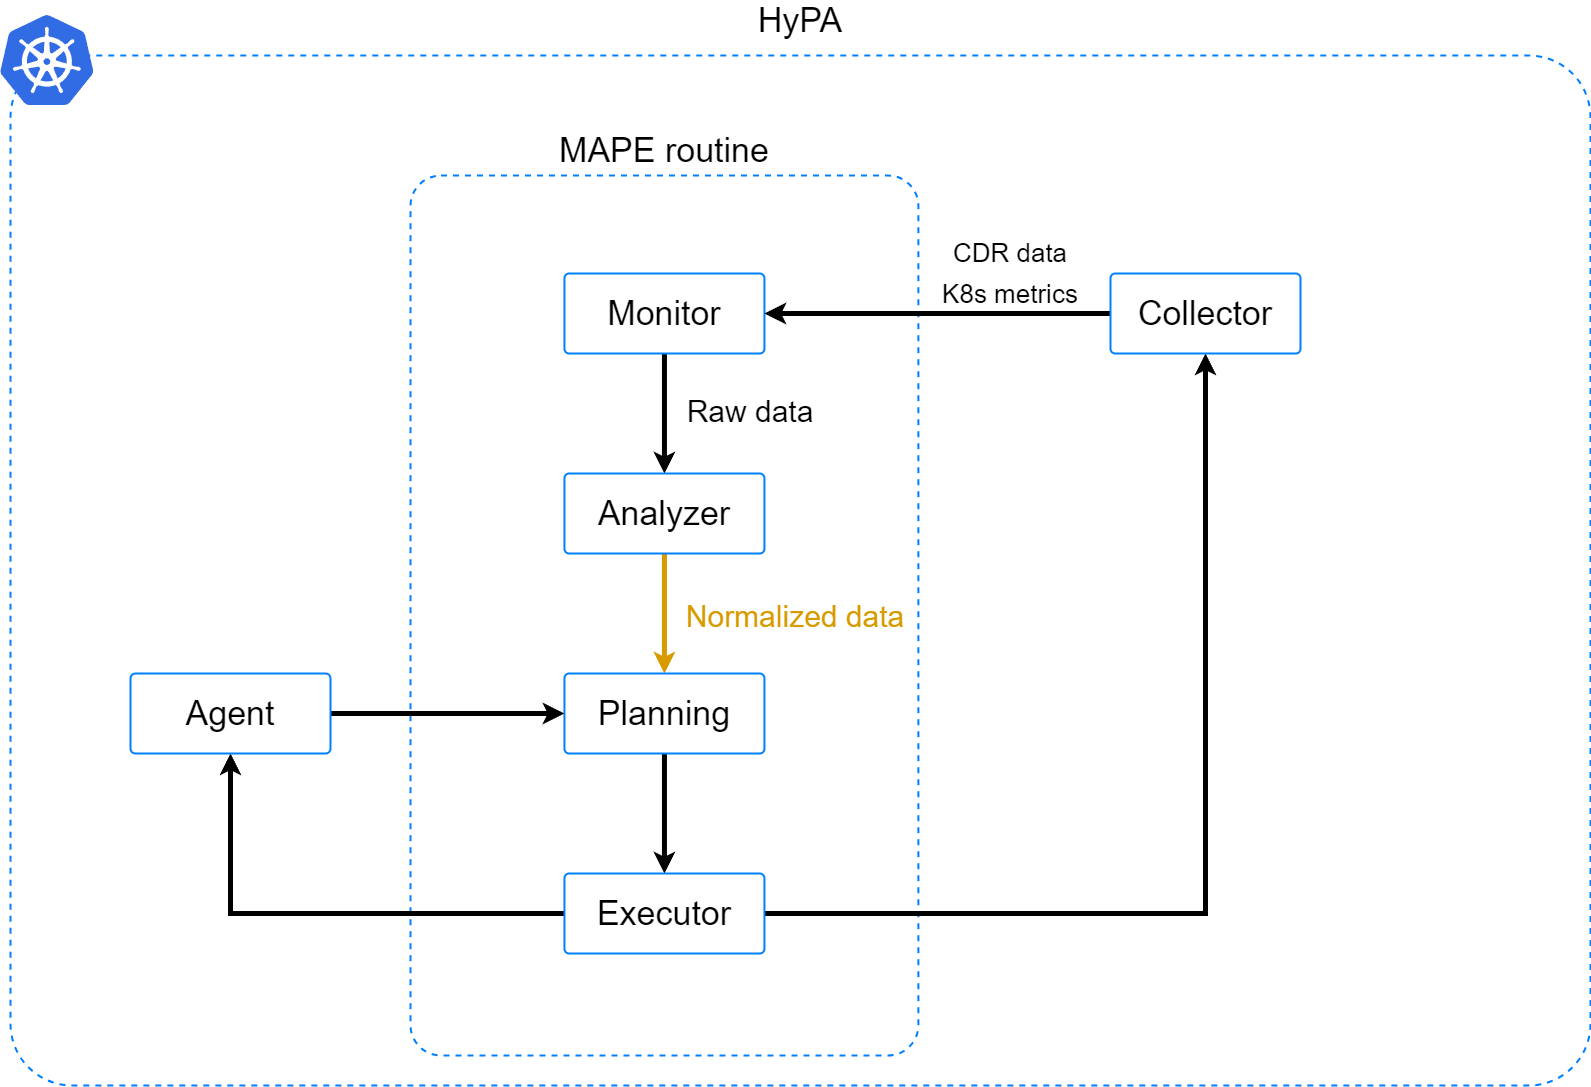
\includegraphics[width=12cm,height=7cm]{_images/trainings_model_3.png}
	\end{figure}
\end{frame}

\begin{frame}
	\frametitle{Model Training (5)}
	
	\begin{figure}
		\centering
		\vspace*{-0.4cm}
		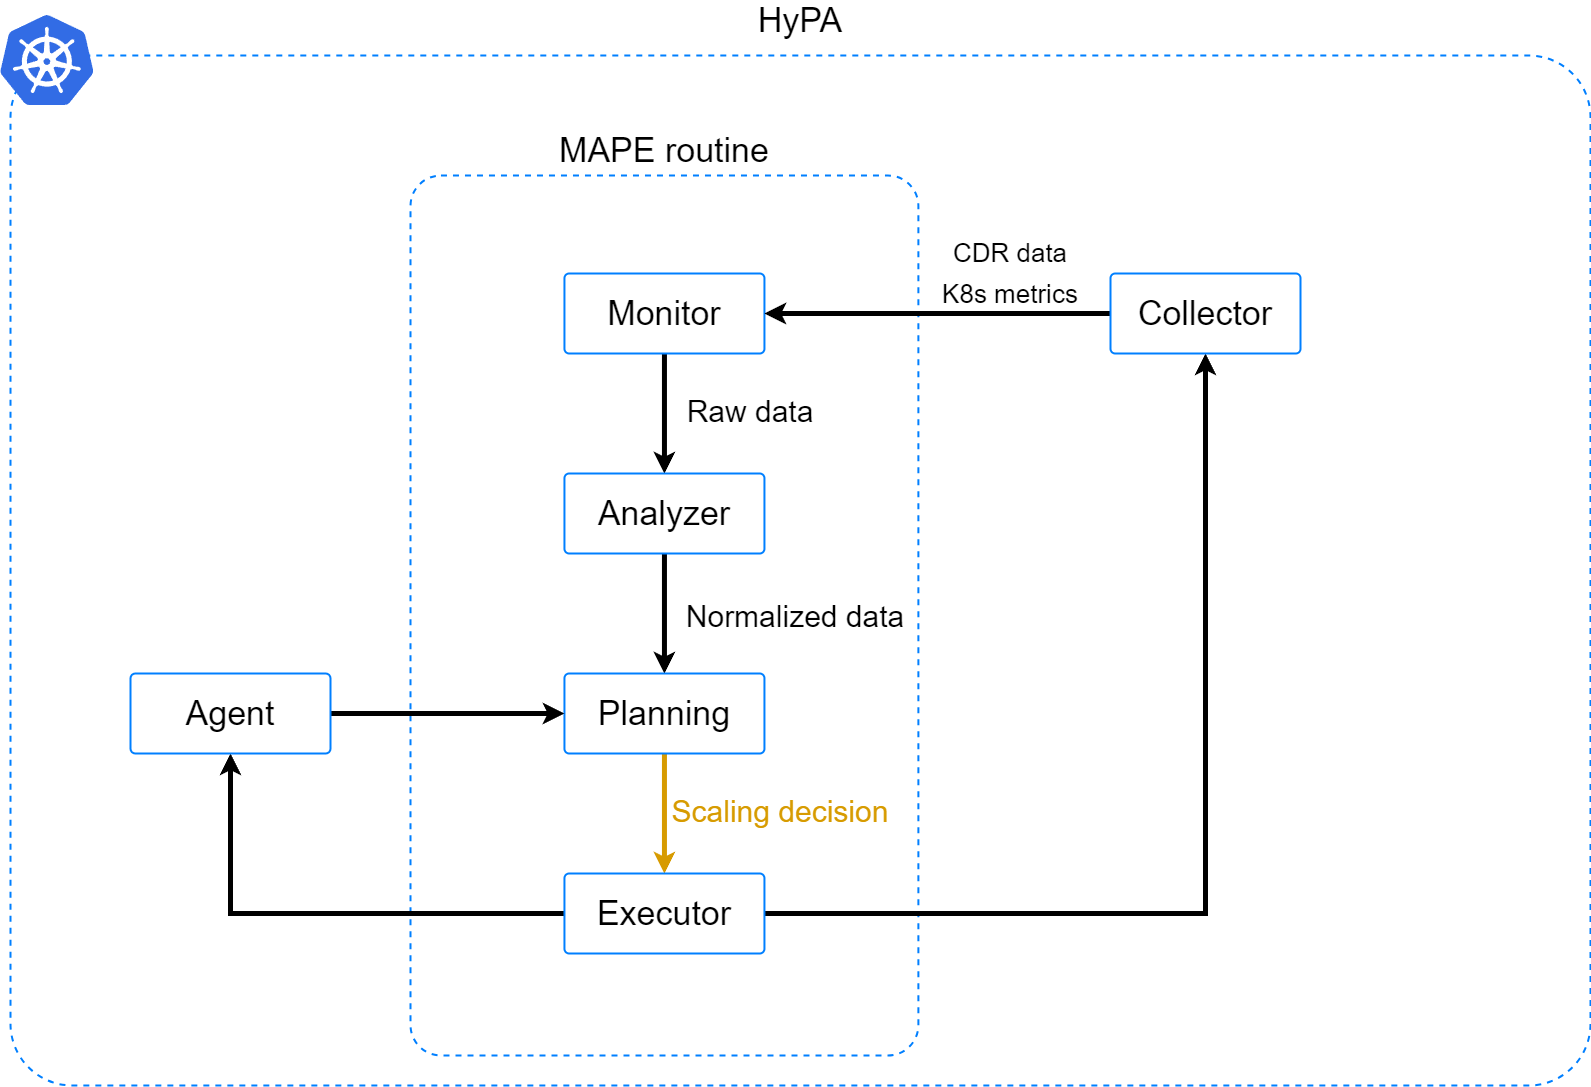
\includegraphics[width=12cm,height=7cm]{_images/trainings_model_4.png}
	\end{figure}
\end{frame}

\begin{frame}
	\frametitle{Model Training (6)}
	
	\begin{figure}
		\centering
		\vspace*{-0.4cm}
		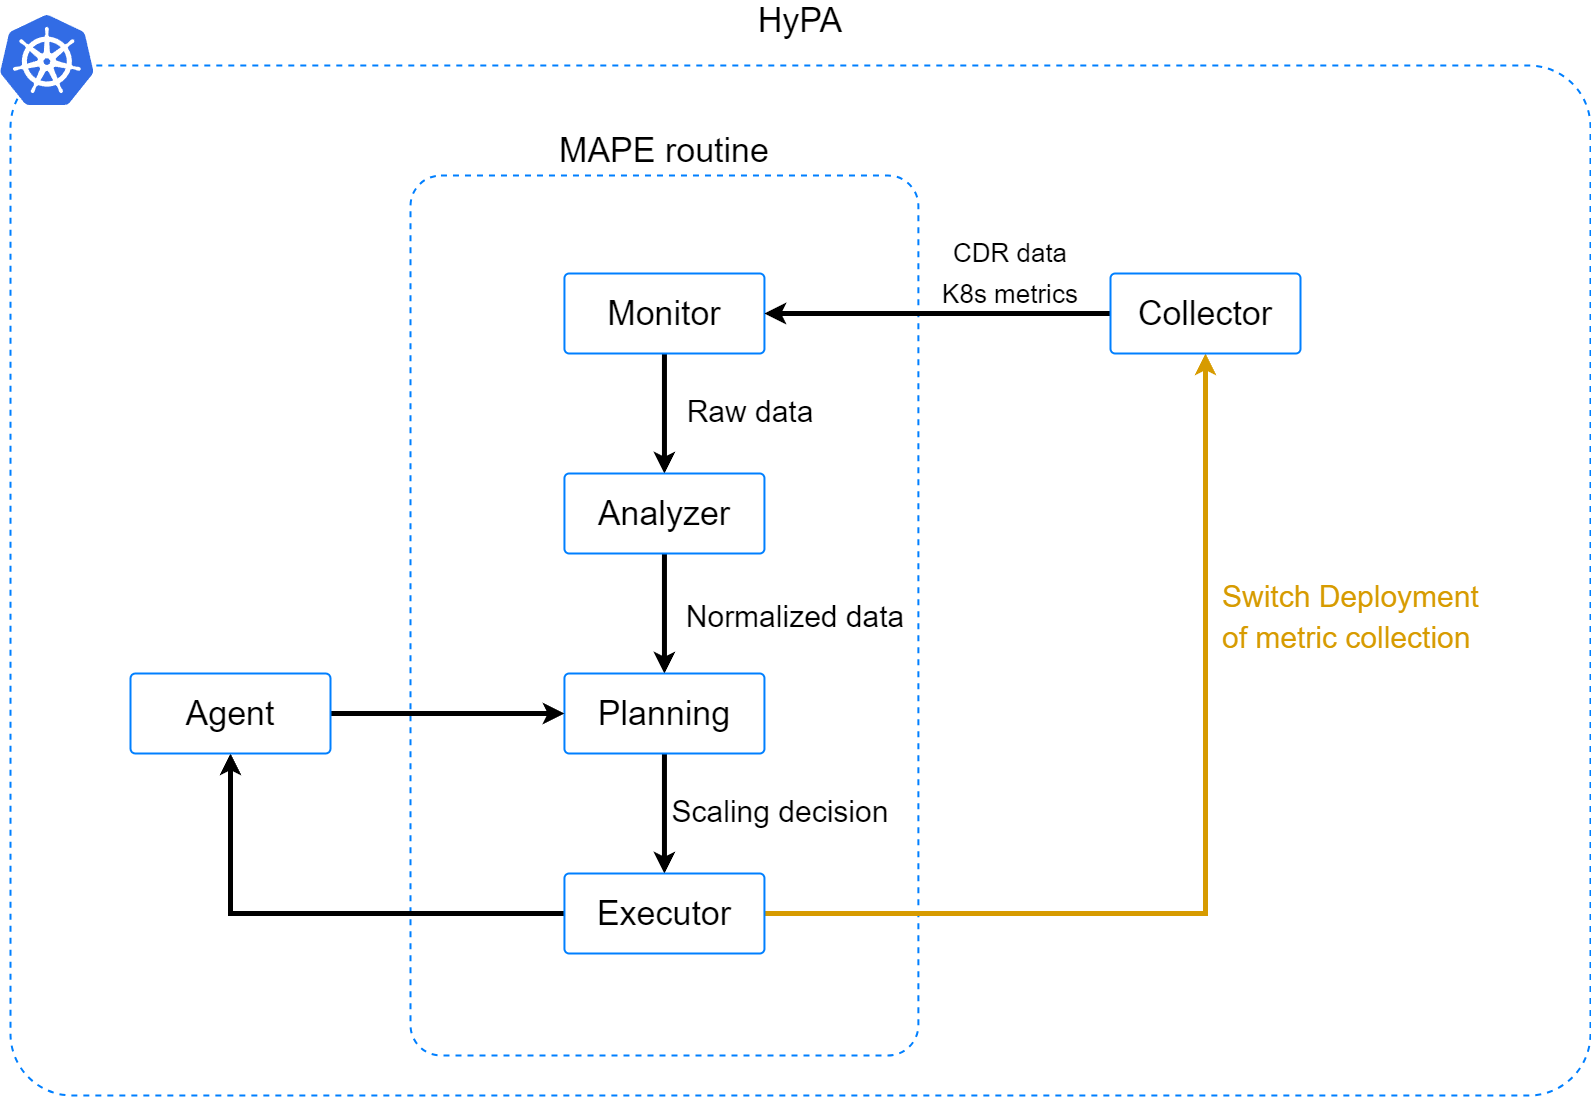
\includegraphics[width=12cm,height=7cm]{_images/trainings_model_5.png}
	\end{figure}
\end{frame}

\begin{frame}
	\frametitle{Model Training (7)}
	
	\begin{figure}
		\centering
		\vspace*{-0.4cm}
		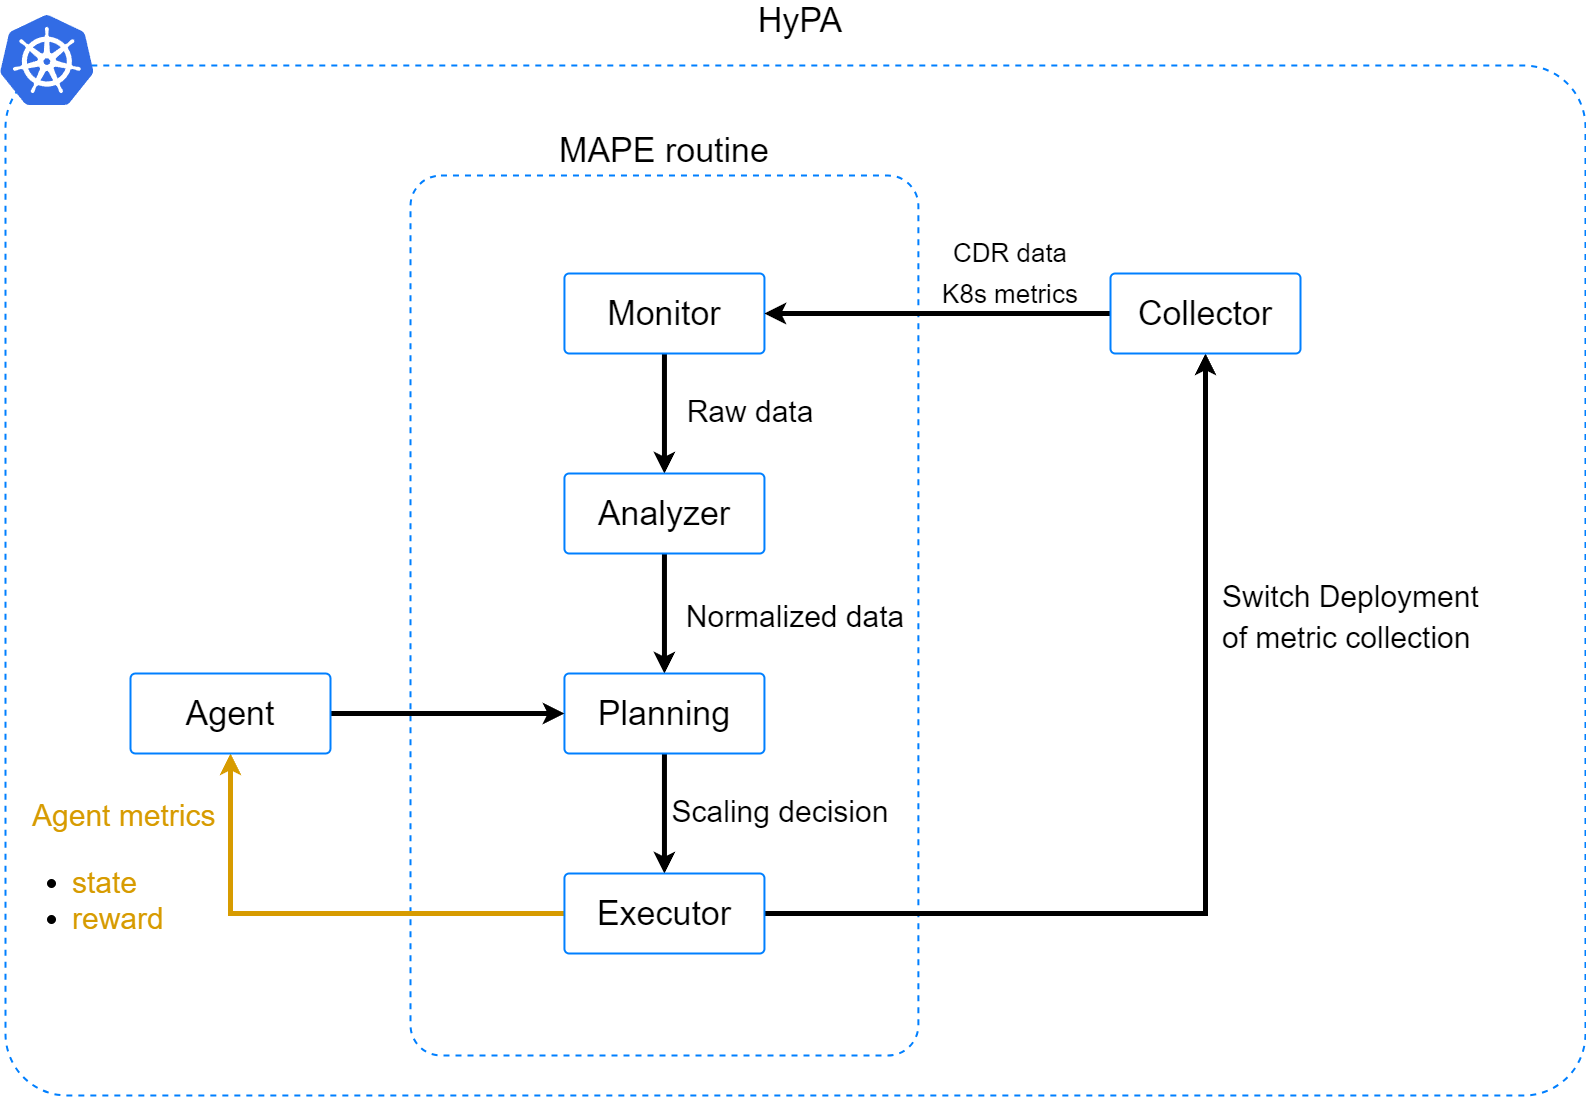
\includegraphics[width=12cm,height=7cm]{_images/trainings_model_6.png}
	\end{figure}
\end{frame}

\begin{frame}
	\frametitle{Model Training (8)}
	
	\begin{figure}
		\centering
		\vspace*{-0.4cm}
		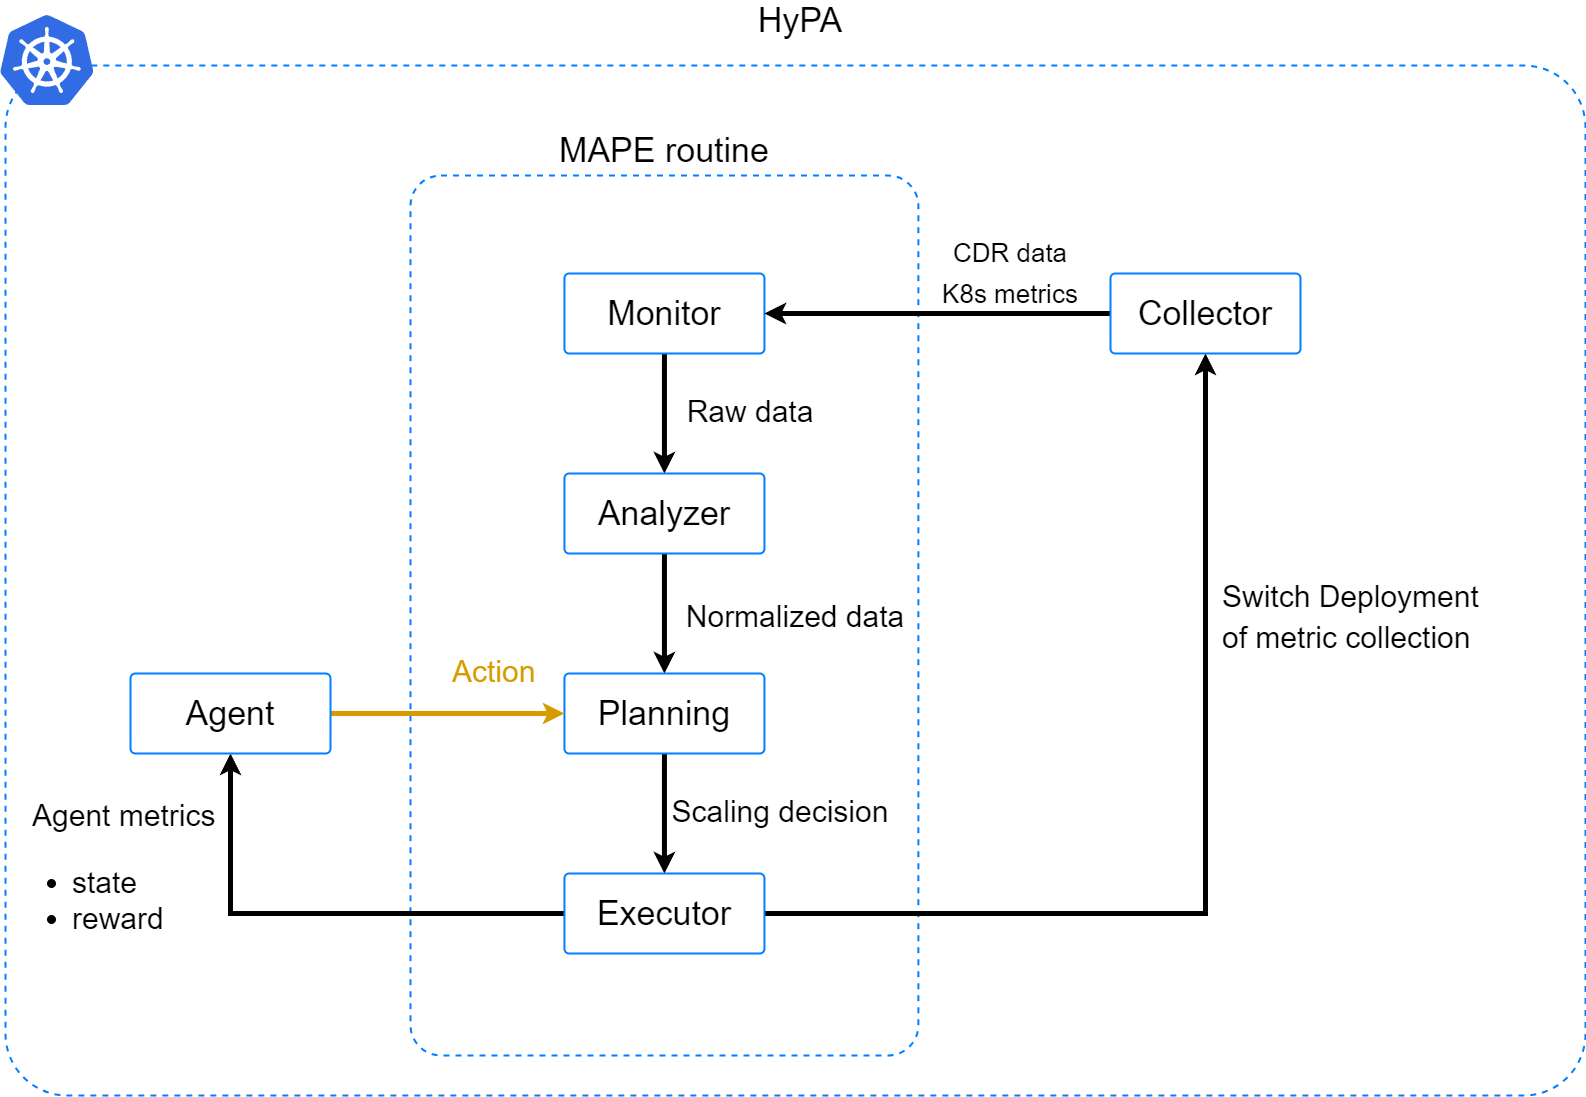
\includegraphics[width=12cm,height=7cm]{_images/trainings_model_7.png}
	\end{figure}
\end{frame}

\begin{frame}
	\frametitle{RL Training Disadvantage}
	
	\begin{alertblock}{Training duration}
		\begin{itemize}
			\item Time-consuming tasks:
			\begin{itemize}
				\item Scaling operation
				\item Environment response
				\item Data collection
			\end{itemize}
			\item Significant delay after every agent decision (step)
			\item Limits training rate of model
		\end{itemize}
	\end{alertblock}
\end{frame}

\begin{frame}
	\frametitle{RL Training Disadvantage}
	
	\begin{alertblock}{Training duration}
		\begin{itemize}
			\item Time-consuming tasks:
			\begin{itemize}
				\item Scaling operation
				\item Environment response
				\item Data collection
			\end{itemize}
			\item Significant delay after every agent decision (step)
			\item Limits training rate of model
		\end{itemize}
	\end{alertblock}
	
	\begin{block}{Problem}
		\begin{itemize}
			\item Development and retraining time consuming
			\item Significant training duration reduction needed
		\end{itemize}
	\end{block}
\end{frame}


\begin{frame}
	\frametitle{RL Training Optimization}
	
	\begin{alertblock}{Analytical Model}
		\begin{itemize}
			\item Finite scaling options covering WD's cases
			\item Deploying all scaling options
			\item Same workload everywhere
			\item Only metric collection switched
		\end{itemize}
	\end{alertblock}
\end{frame}

\begin{frame}
	\frametitle{RL Training Optimization}
	
	\begin{alertblock}{Analytical Model}
		\begin{itemize}
			\item Finite scaling options covering WD's cases
			\item Deploying all scaling options
			\item Same workload everywhere
			\item Only metric collection switched
		\end{itemize}
	\end{alertblock}
	
	\begin{block}{Improvement}
		\begin{itemize}
			\item Faster environment response
			\item Broader agent decision exploration
			\item Training three times faster
		\end{itemize}
	\end{block}
\end{frame}

\subsection{Evaluation}

\begin{frame}
	\frametitle{Evaluation HyPA}
	
	\begin{figure}
		\centering
		\vspace*{-0.4cm}
		\includegraphics[width=12cm,height=7cm]{_images/evaluation_model.png}
	\end{figure}
\end{frame}


\begin{frame}
	\frametitle{Evaluation Competitors}
	
	\begin{block}{Horizontal Pod Autoscaler (HPA)}
		\begin{itemize}
			\item Kubernetes default
			\item Threshold based
			\item Reactive autoscaler
			\item No expert knowledge for setup
		\end{itemize}
	\end{block}
\end{frame}

\begin{frame}
	\frametitle{Evaluation Competitors}
	
	\begin{block}{Horizontal Pod Autoscaler (HPA)}
		\begin{itemize}
			\item Kubernetes default
			\item Threshold based
			\item Reactive autoscaler
			\item No expert knowledge for setup
		\end{itemize}
	\end{block}
	
	\begin{block}{Multi-Objective-Hybrid-Autoscaling (MOHA)}
		\begin{itemize}
			\item Machine Learning based (NN, SVM, LR)
			\item Hybrid scaling
			\item Code modifications to support usecase
		\end{itemize}
	\end{block}
\end{frame}

\begin{frame}
	\frametitle{Evaluation Scenarios}
	
	\begin{alertblock}{Call Volume Groups}
		\begin{table}
			\begin{center}
				\begin{tabular}{|c c c|}
					\hline
					Group & Call volume & Client share \\
					\hline
					light & $< 10^4$ & 31.99 \% \\
					medium & $10^4 - 10^5$ & 53.02 \% \\
					heavy &  $10^5 - 10^6$ & 14.34 \% \\
					very heavy & $\ge 10^6$ & 0.65 \% \\
					\hline
				\end{tabular}
			\end{center}
		\end{table}
	\end{alertblock}
\end{frame}

\begin{frame}
	\frametitle{Evaluation Scenarios}
	
	\begin{alertblock}{Call Volume Groups}
		\begin{table}
			\begin{center}
				\begin{tabular}{|c c c|}
					\hline
					Group & Call volume & Client share \\
					\hline
					light & $< 10^4$ & 31.99 \% \\
					medium & $10^4 - 10^5$ & 53.02 \% \\
					heavy &  $10^5 - 10^6$ & 14.34 \% \\
					very heavy & $\ge 10^6$ & 0.65 \% \\
					\hline
				\end{tabular}
			\end{center}
		\end{table}
	\end{alertblock}
	
	\begin{block}{Scenarios}
		\begin{enumerate}
			\item Random common client
			\item Averaged call volume per group
		\end{enumerate}
	\end{block}
\end{frame}

\begin{frame}
	\frametitle{Scenario 1 Visualization}
	\begin{figure}
		\centering
		\vspace*{-0.25cm}
		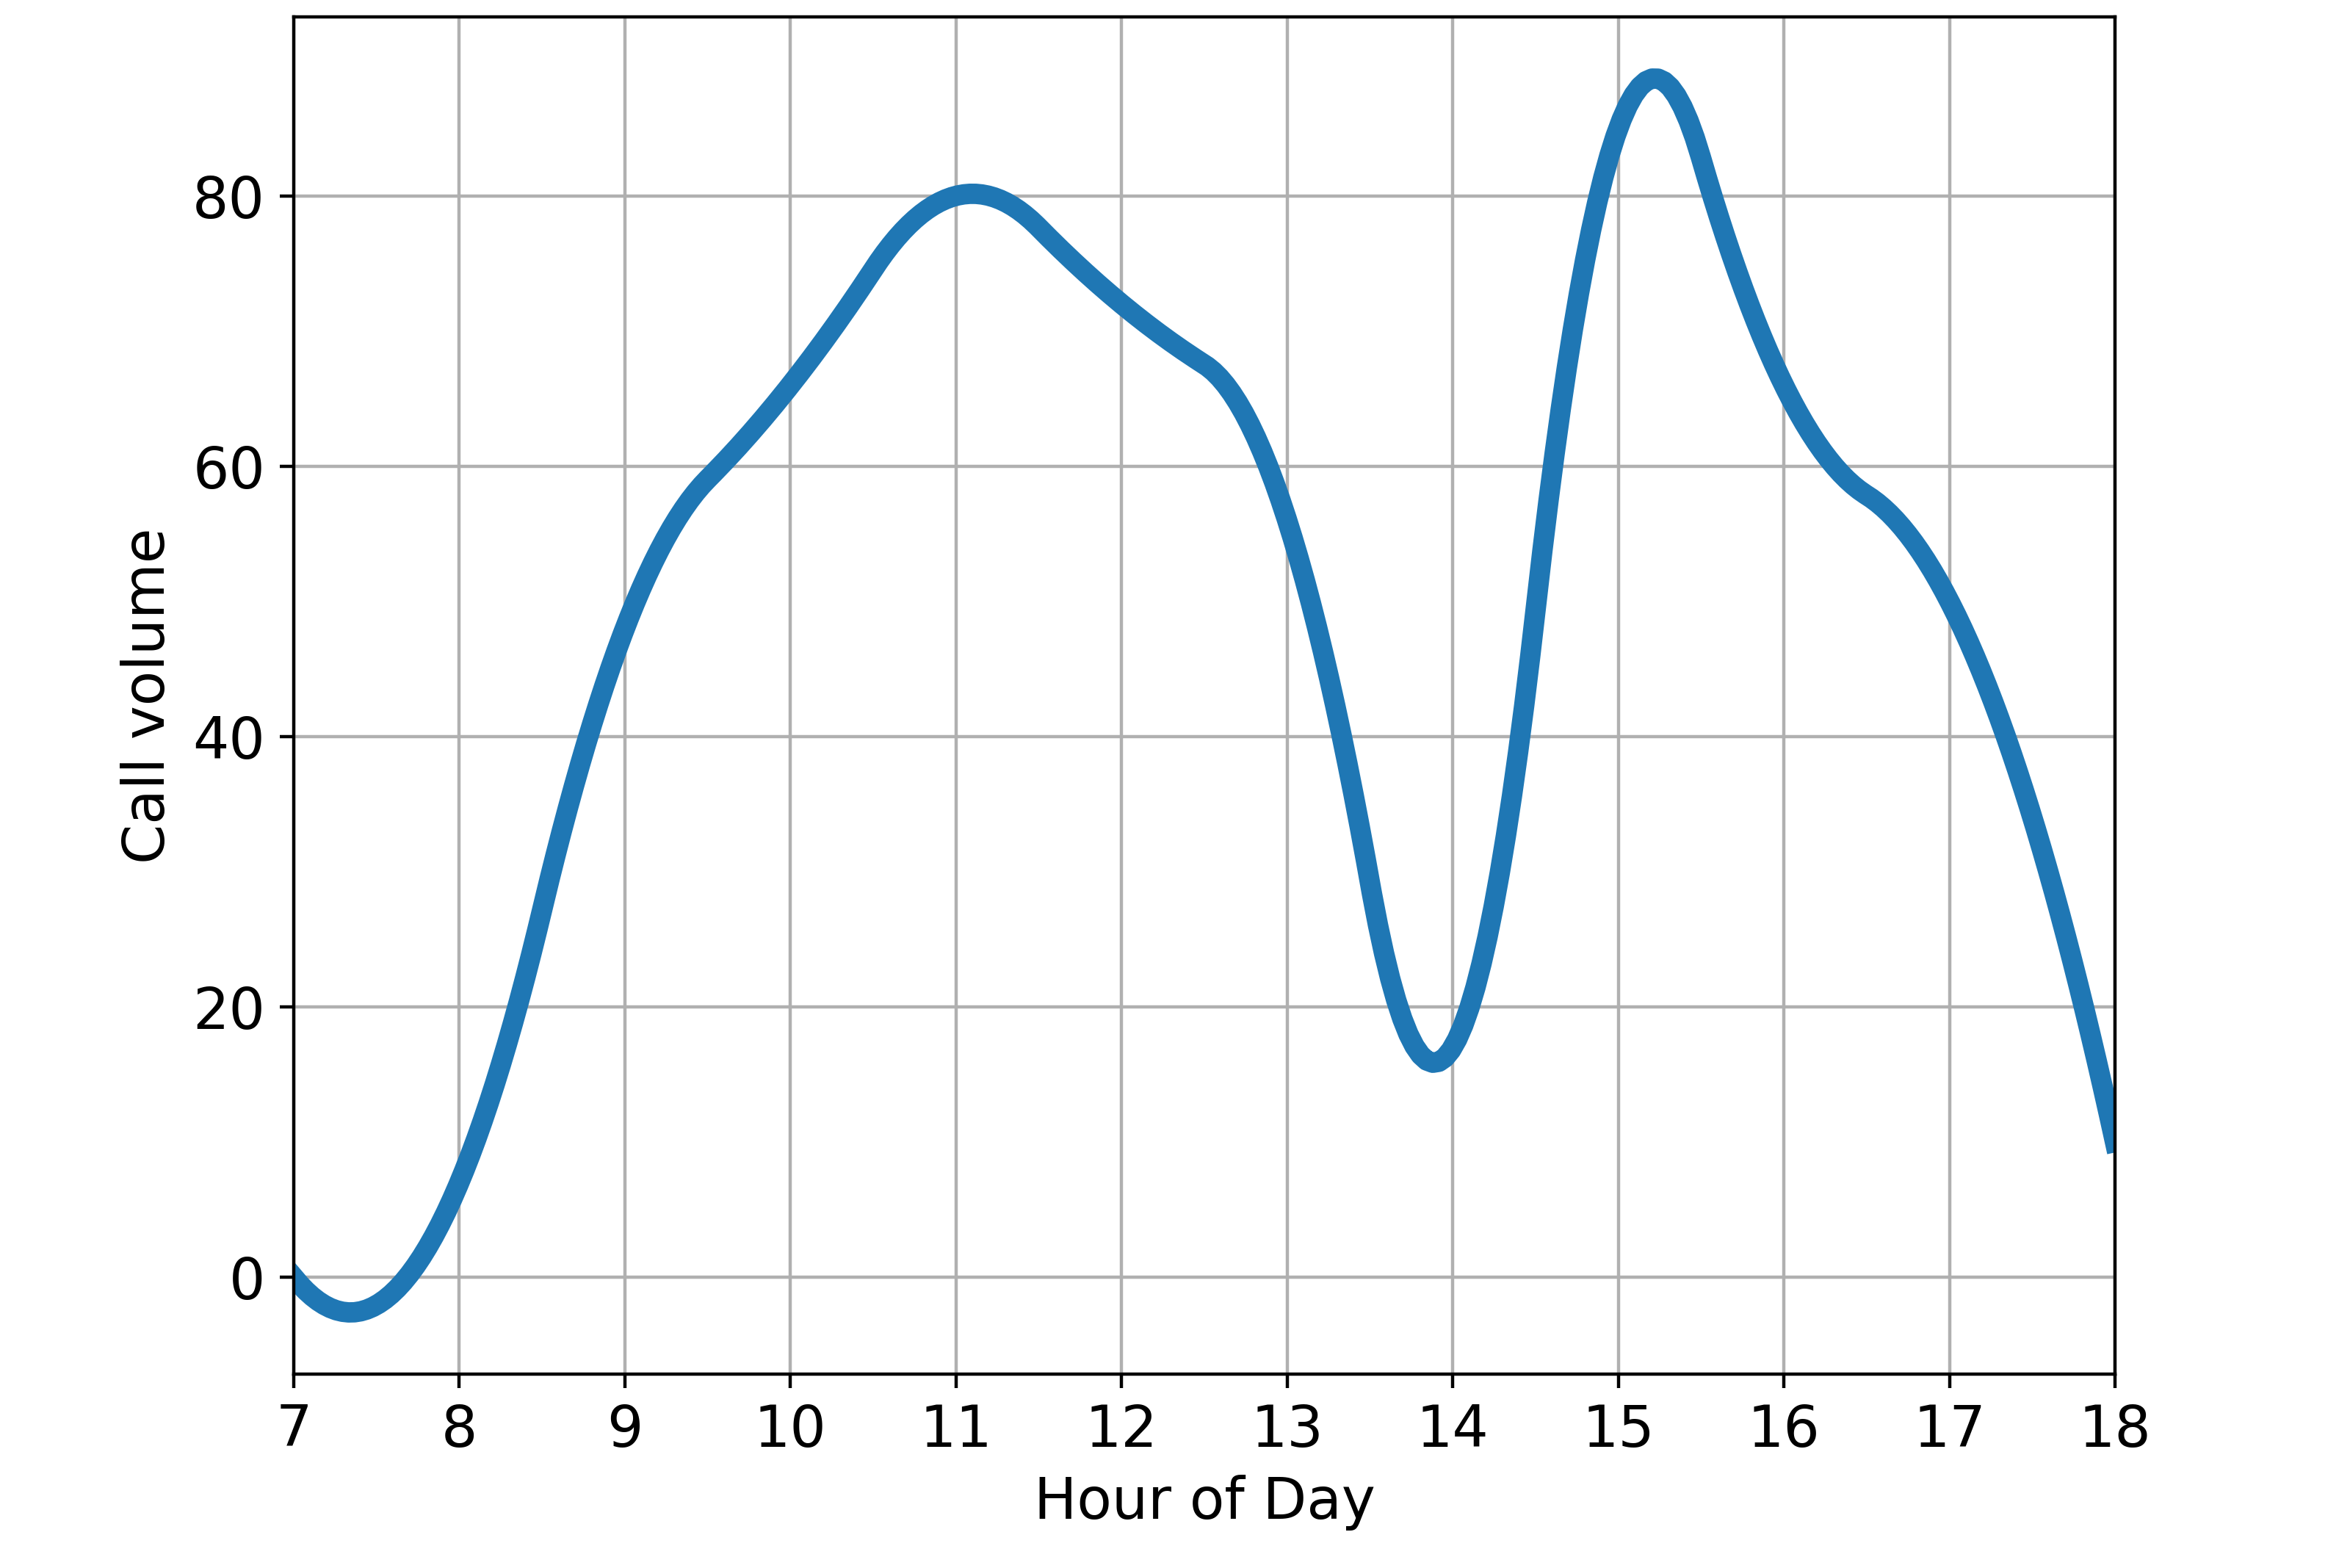
\includegraphics[width=11cm,height=7cm]{_images/scenario_1/call_distribution_real.png}
	\end{figure}
\end{frame}

\begin{frame}
	\frametitle{Scenario 1 Result Calls}
	\begin{figure}
		\centering
		\vspace*{-0.5cm}
		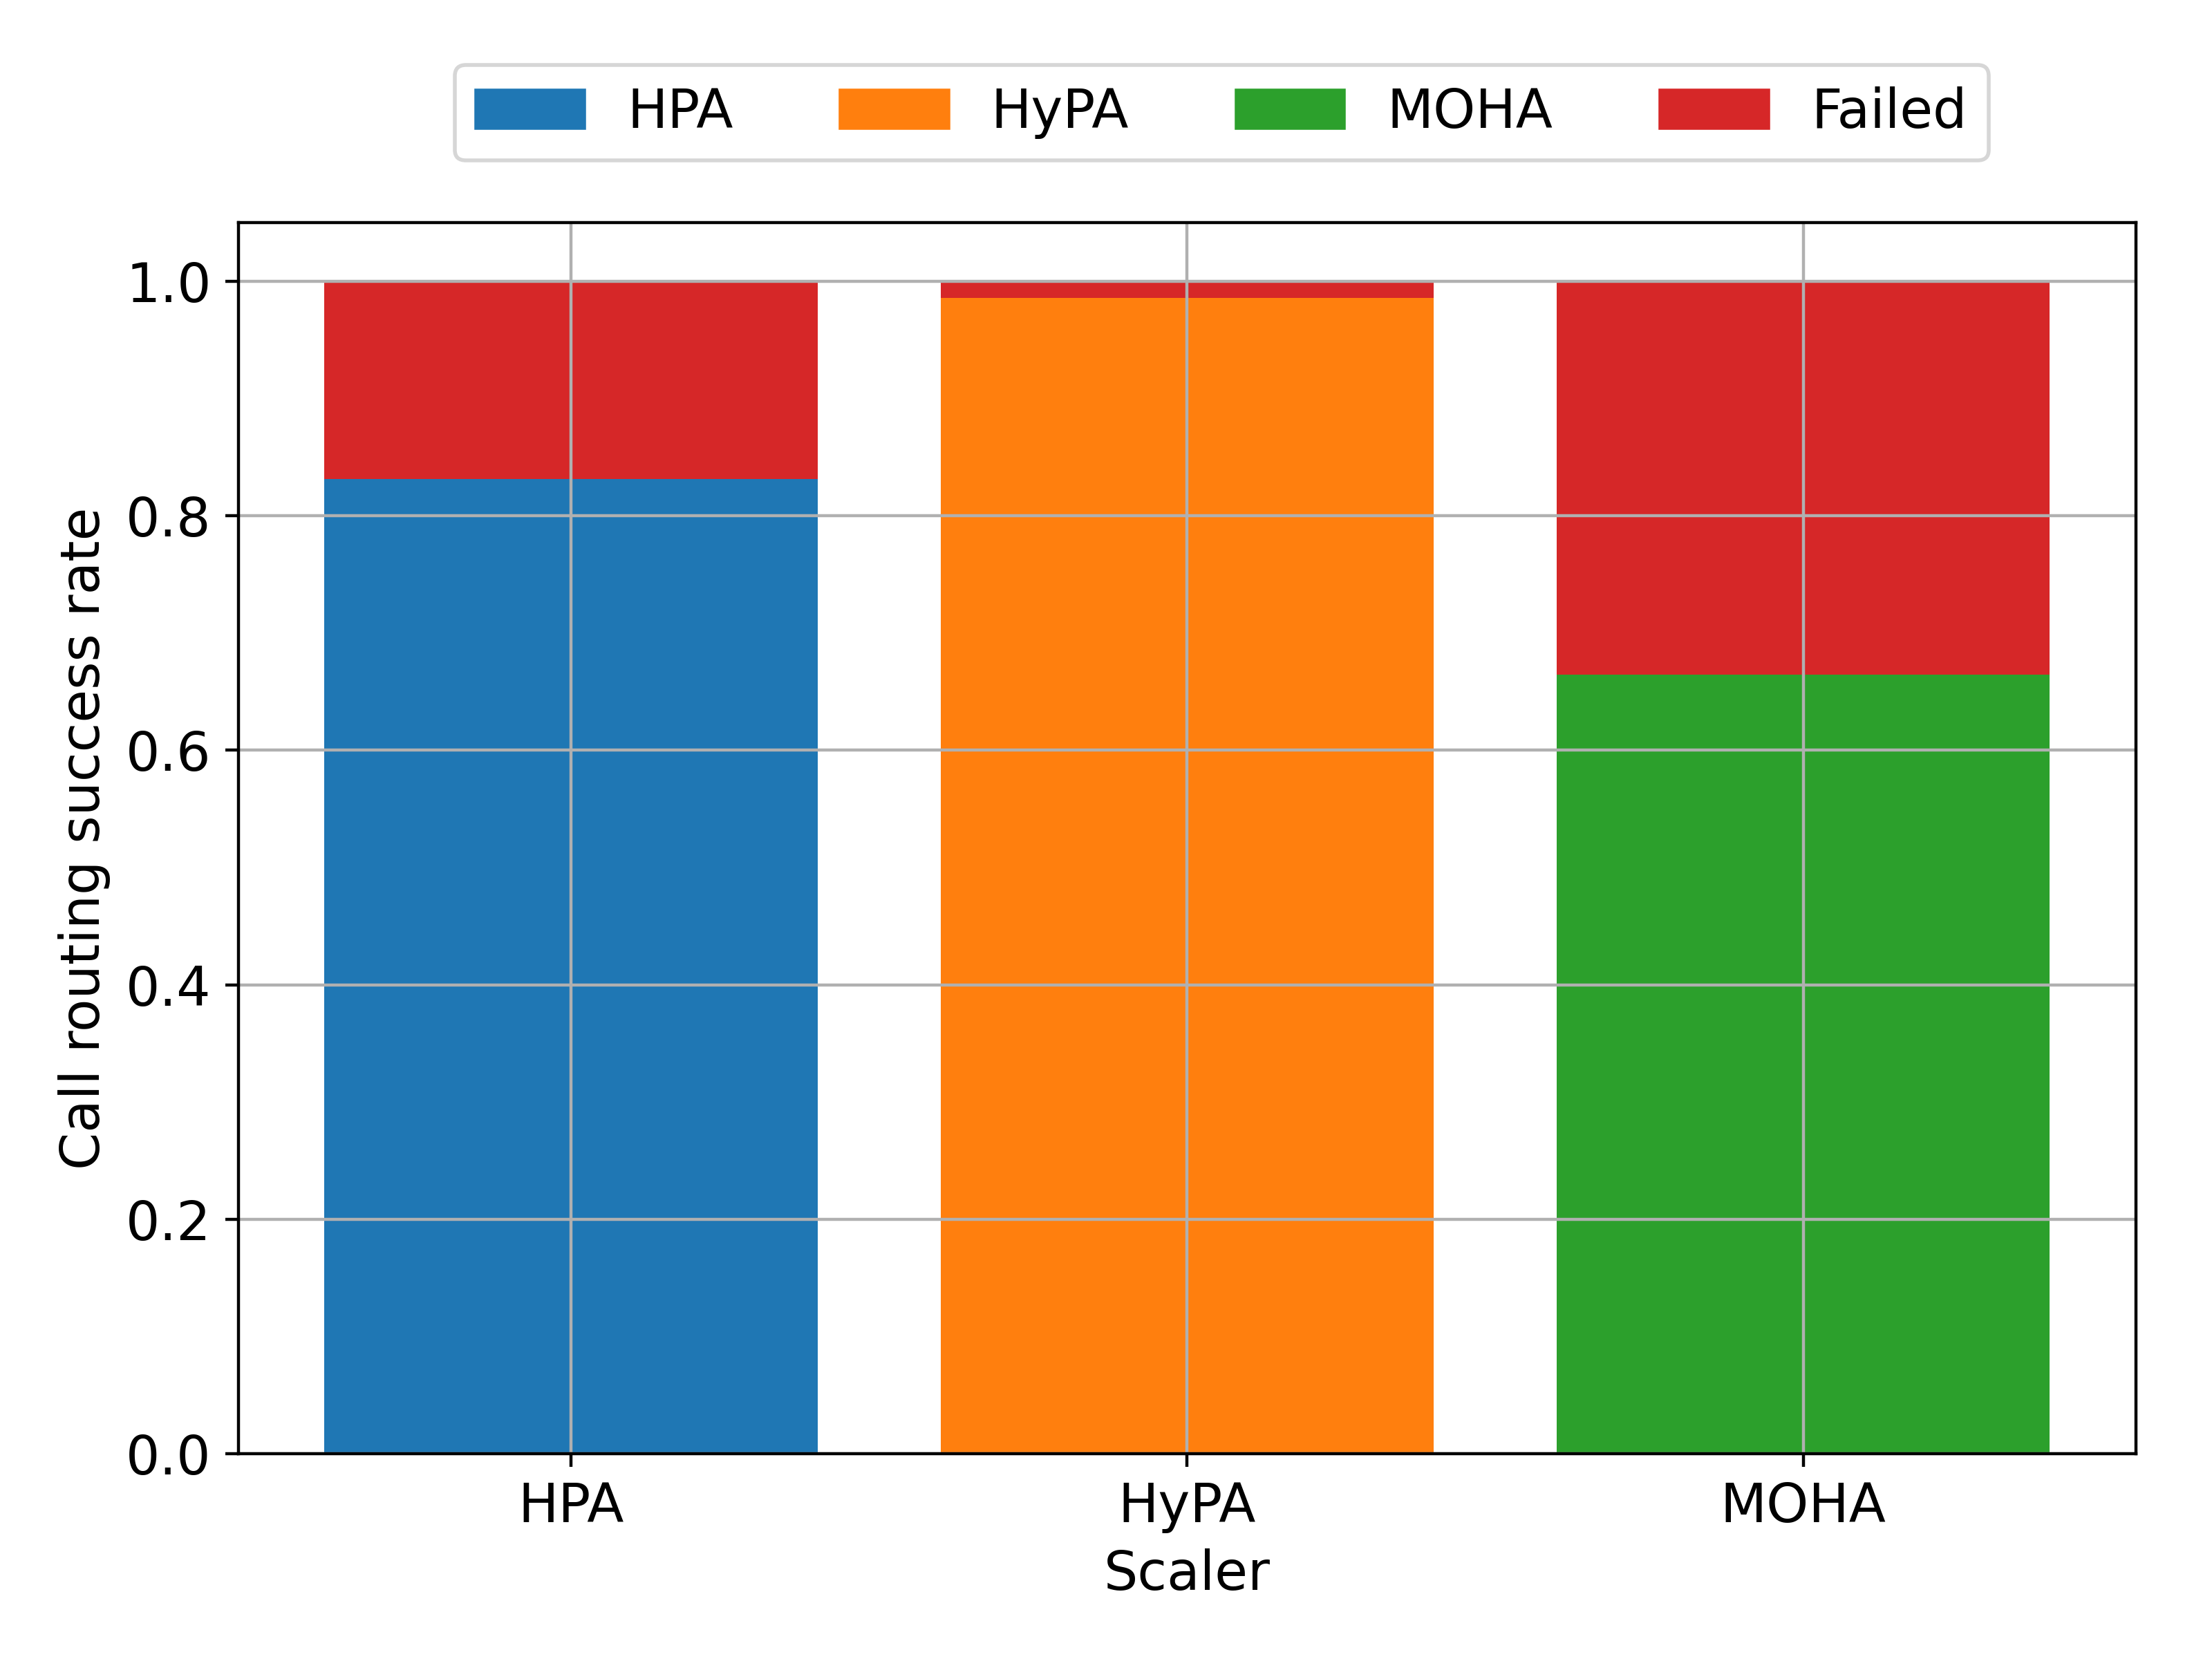
\includegraphics[width=11cm,height=7.4cm]{_images/scenario_1/call_comparison.png}
	\end{figure}
\end{frame}

\begin{frame}
	\frametitle{Scenario 1 Result Latency}
	\begin{figure}
		\centering
		\vspace*{-0.5cm}
		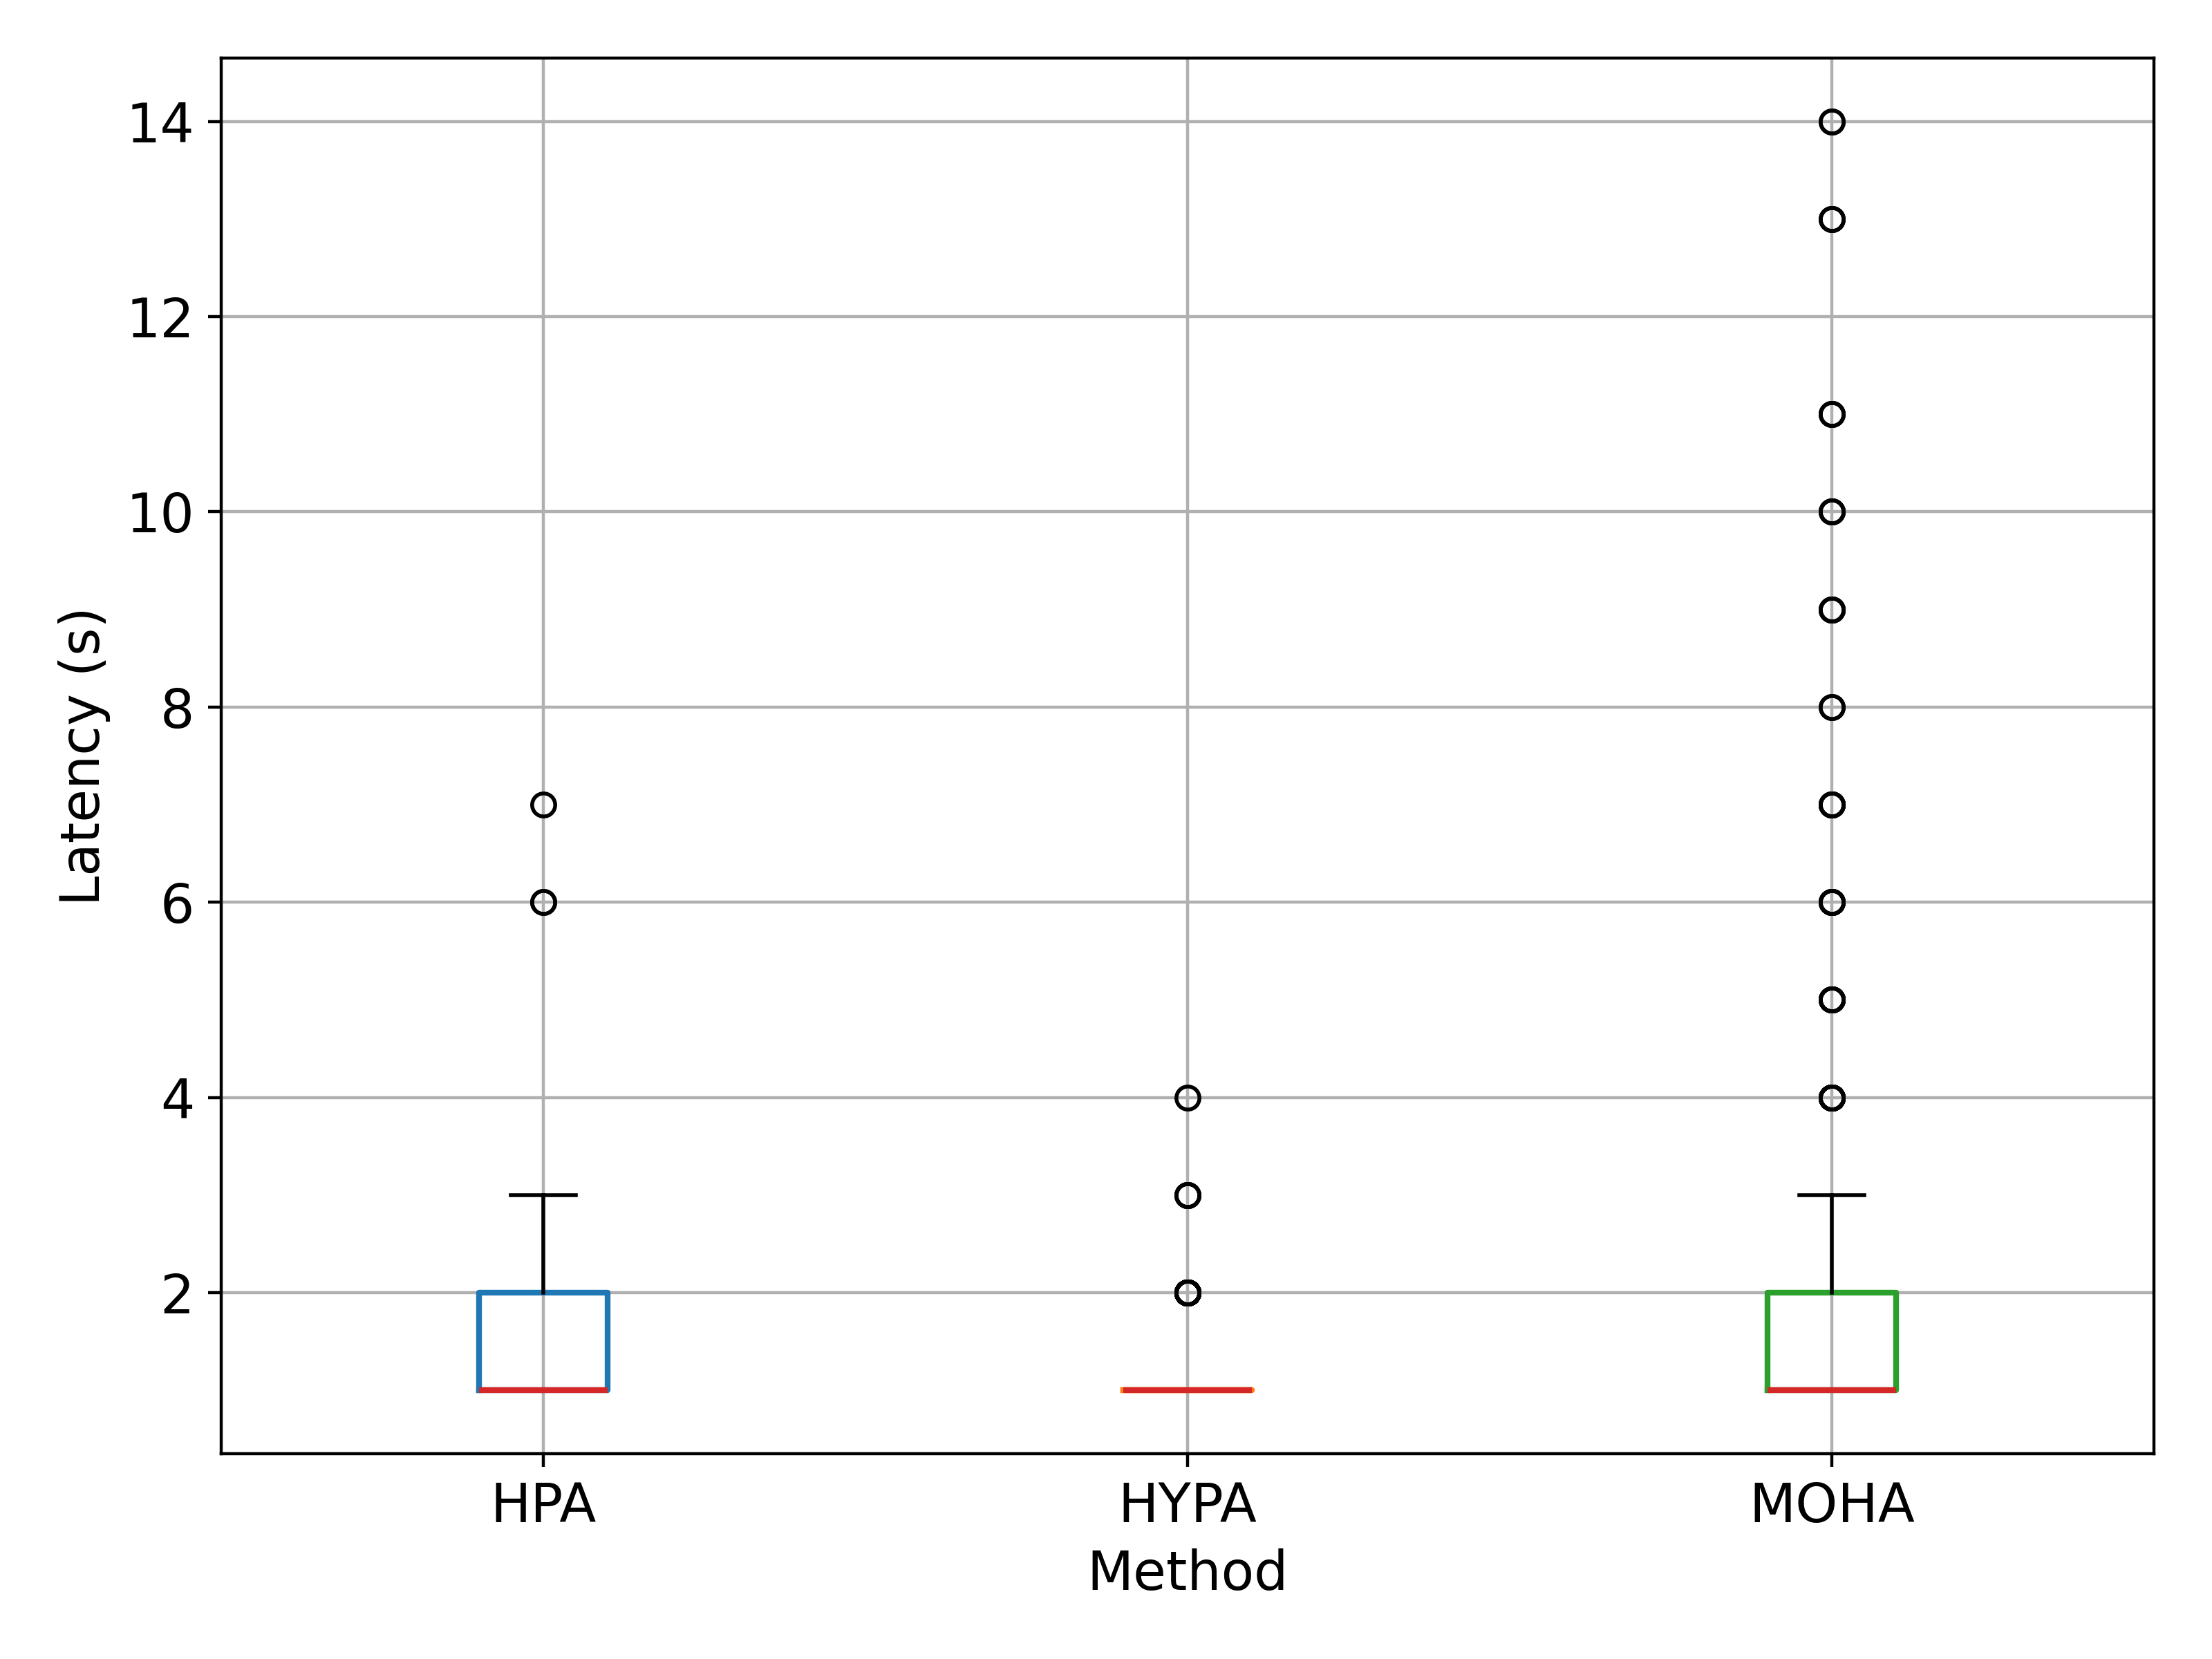
\includegraphics[width=11cm,height=7.4cm]{_images/scenario_1/latency.png}
	\end{figure}
\end{frame}

\begin{frame}
	\frametitle{Scenario 2 Visualization}
		\begin{table}
			\vspace{-0.5cm}
			\begin{center}
				\resizebox{!}{3.7cm}{%
				\begin{tabular}{|c c c c c|}
					\hline
					Hour & light  & medium & heavy & very heavy \\
					\hline
					7 & 1 & 3 & 51 & 984 \\
					8 & 2 & 7 & 159 & 3069 \\
					9 & 2 & 9 & 193 & 4187 \\
					10 & 2 & 9 & 191 & 7196 \\
					11 & 2 & 8 & 175 & 3901 \\
					12 & 1 & 4 & 91 & 2468 \\
					13 & 1 & 6 & 128 & 3058 \\
					14 & 1 & 6 & 127 & 3025 \\
					15 & 1 & 5 & 109 & 2901 \\
					16 & 1 & 3 & 75 & 1803 \\
					17 & 1 & 2 & 36 & 726 \\
					\hline
					Client share & 31.99\% & 53.02\% & 14.34\% & 0.65\% \\
					\hline
				\end{tabular}}
			\end{center}
		\end{table}
\end{frame}

\begin{frame}
	\frametitle{Scenario 2 Result Calls}
	\begin{figure}
		\centering
		\vspace*{-0.5cm}
		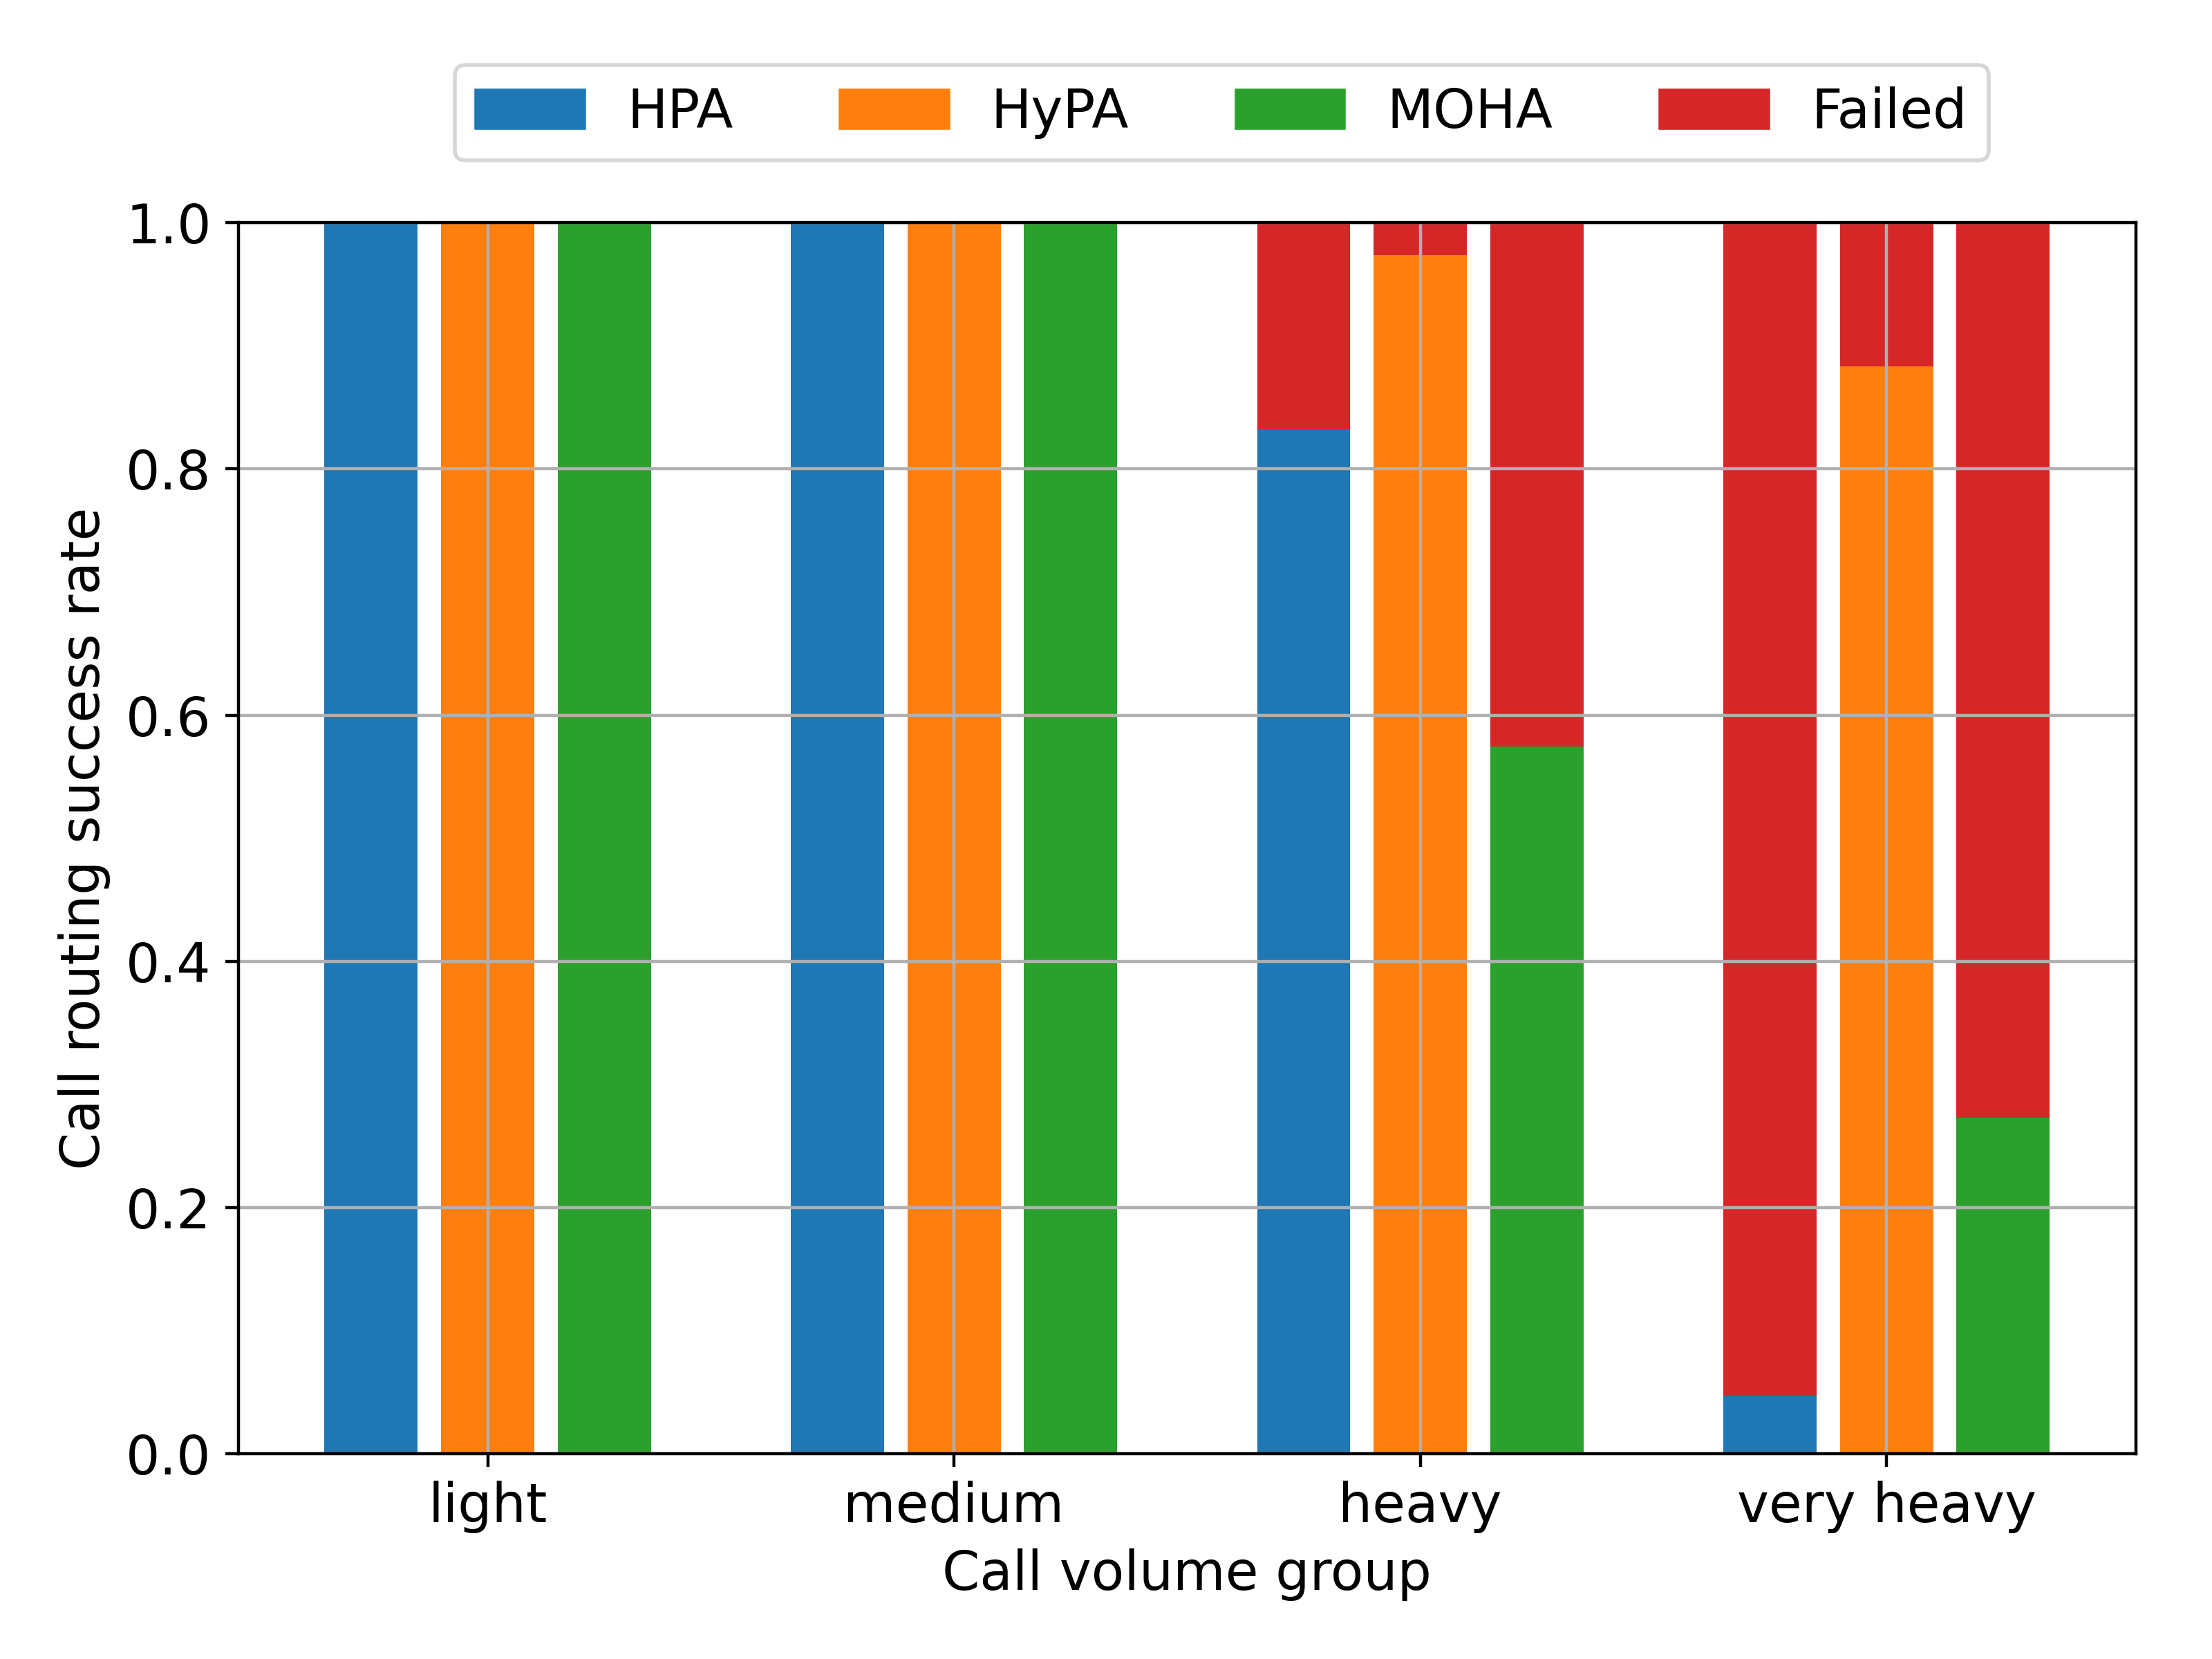
\includegraphics[width=11cm,height=7.4cm]{_images/scenario_2/call_comparison_stacked.png}
	\end{figure}
\end{frame}

\begin{frame}
	\frametitle{Scenario 2 Result Latency}
	\begin{figure}
		\centering
		\vspace*{-0.5cm}
		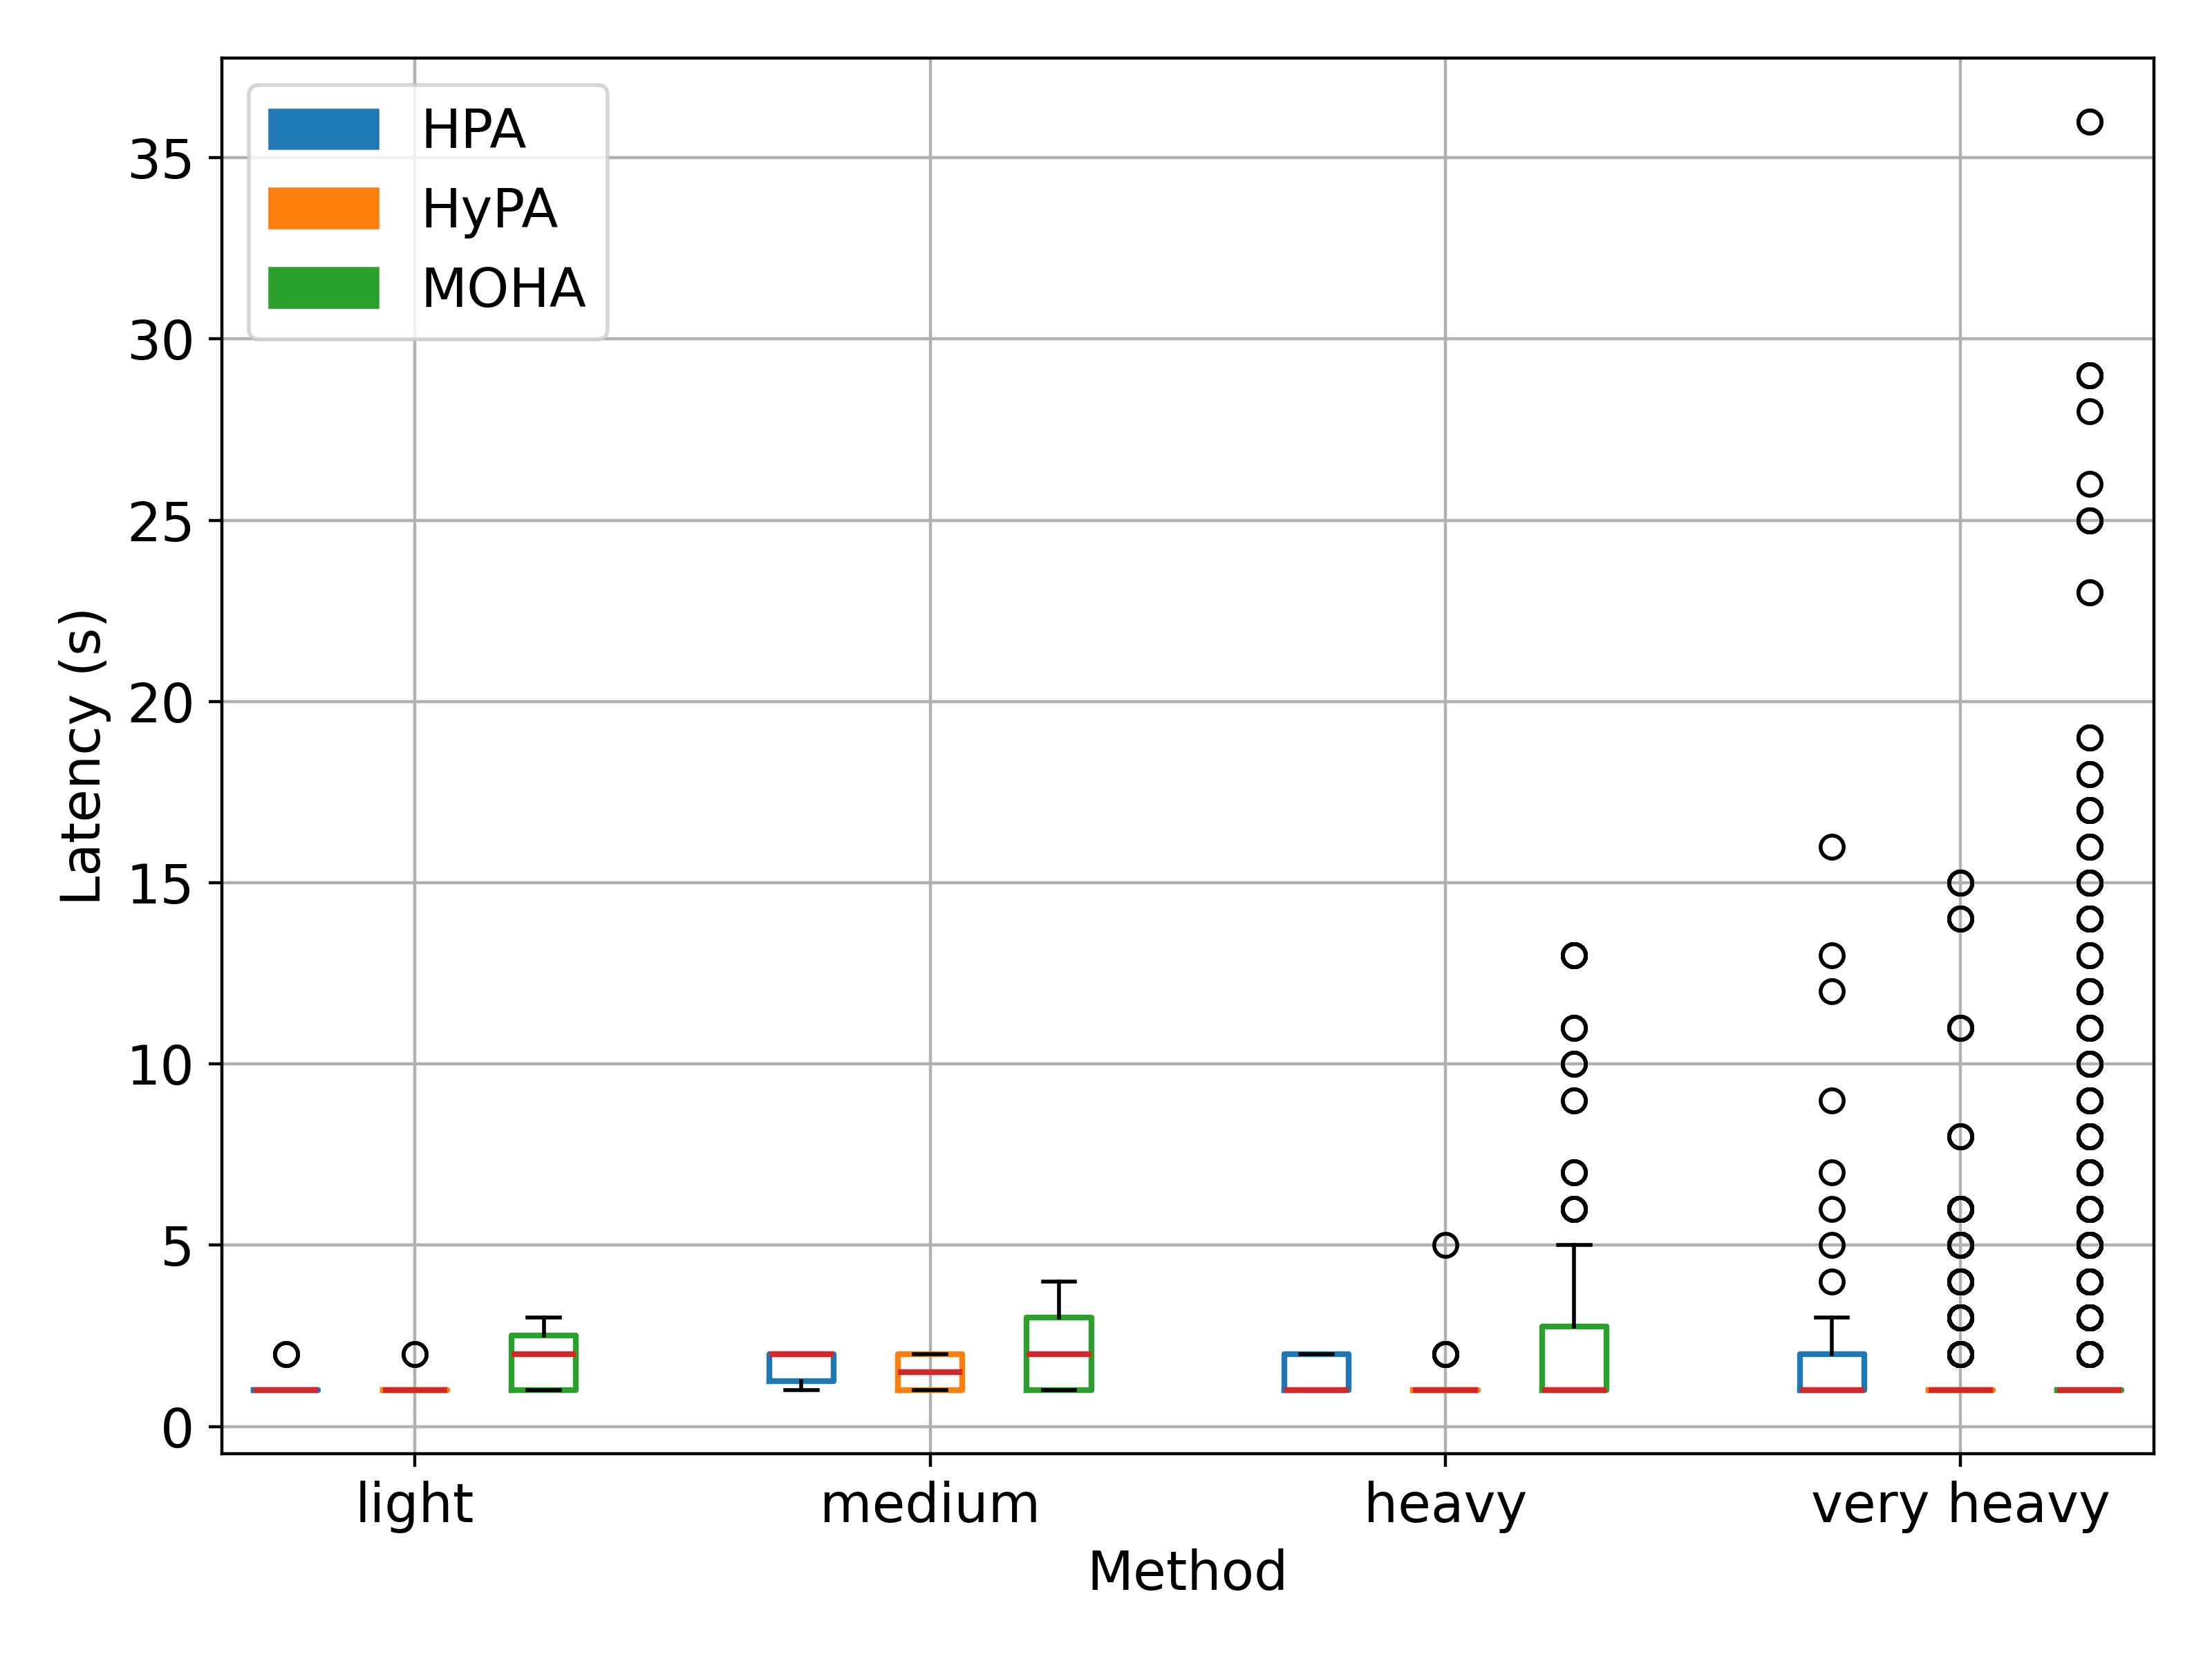
\includegraphics[width=11cm,height=7.4cm]{_images/scenario_2/latency_stacked.png}
	\end{figure}
\end{frame}

\subsection{Project Timeline}
\begin{frame}
	\begin{figure}
		\centering
		\vspace*{-0.2cm}
		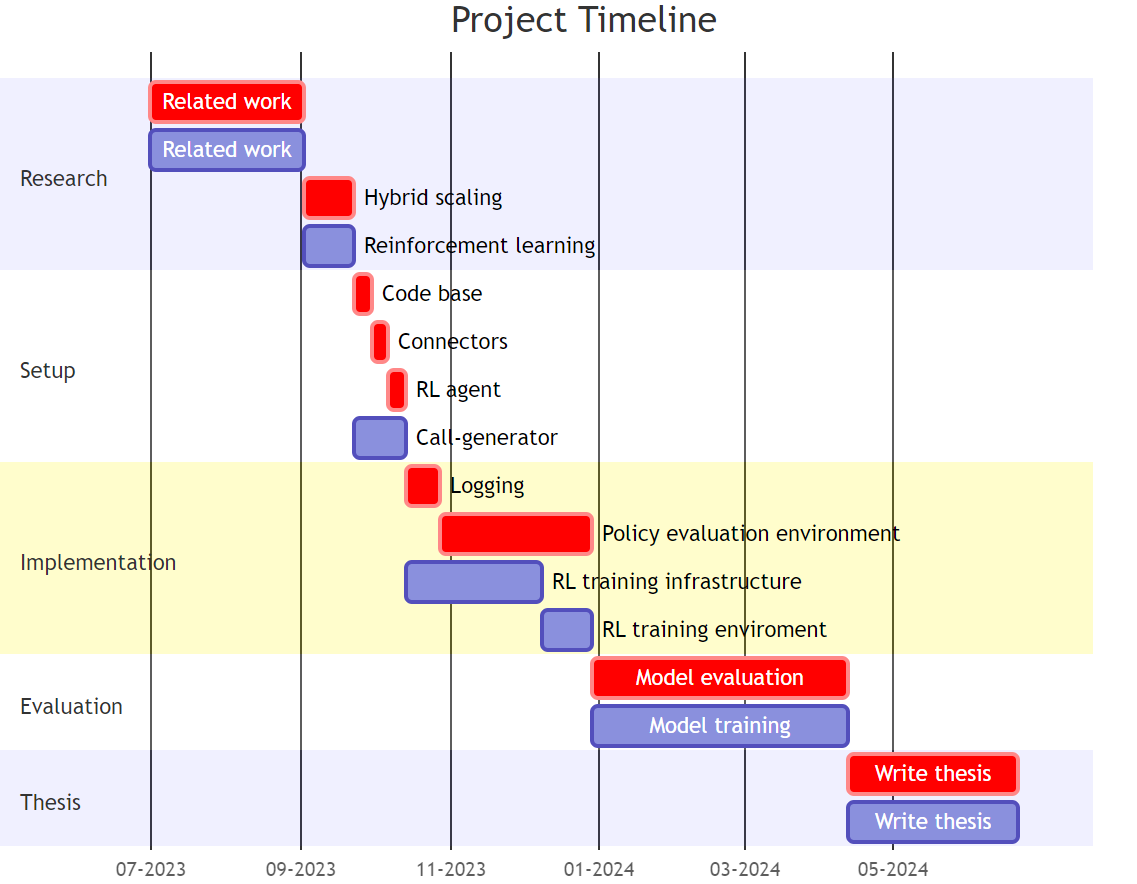
\includegraphics[width=13cm,height=8cm]{_images/milestones.png}
	\end{figure}
\end{frame}


\subsection{References}
\begin{frame}[allowframebreaks]
	\frametitle{References}
	
	\nocite{bib_uibk_latex}
	
	\bibliographystyle{unsrt}
	\bibliography{main.bib}
\end{frame}


\end{document}